\documentclass[12pt]{article}

\usepackage[margin=1in]{geometry}
\usepackage[T1]{fontenc}
\usepackage[utf8]{inputenc}
\usepackage{textcomp}
\usepackage{newtxtext,newtxmath}
\usepackage{amsmath}
\usepackage{graphicx}
\usepackage{booktabs}
\usepackage{array}
\usepackage{longtable}
\usepackage{calc}
\usepackage{float}
\usepackage{caption}
\usepackage{setspace}
\usepackage{lineno}
\usepackage{xcolor}
\usepackage[round,authoryear]{natbib}
\usepackage[bookmarks=false]{hyperref}
\IfFileExists{xurl.sty}{\usepackage{xurl}}{}
\urlstyle{same}

\pagestyle{plain}
\doublespacing
\setlength{\parindent}{0pt}
\setlength{\parskip}{0pt}
\setlength{\emergencystretch}{3em}

\usepackage{titlesec}
\titleformat{\section}
  {\normalfont\large\bfseries}
  {\thesection}{0.75em}{}
\titleformat{\subsection}
  {\normalfont\normalsize\bfseries}
  {\thesubsection}{0.75em}{}
\titleformat{\subsubsection}
  {\normalfont\normalsize\itshape}
  {\thesubsubsection}{0.75em}{}
\titlespacing*{\section}{0pt}{1.2em}{0.6em}
\titlespacing*{\subsection}{0pt}{1.0em}{0.45em}
\titlespacing*{\subsubsection}{0pt}{0.8em}{0.35em}

\newcommand{\tablecaptionfontsize}{\fontsize{10pt}{12pt}\selectfont}
\newcommand{\tablefontsize}{\fontsize{9pt}{11pt}\selectfont}
\DeclareCaptionFont{captionten}{\fontsize{10pt}{12pt}\selectfont}
\captionsetup{
  font=captionten,
  labelfont=bf,
  textfont=captionten,
  justification=raggedright,
  labelsep=period,
  singlelinecheck=false
}
\newcolumntype{L}[1]{>{\tablefontsize\raggedright\arraybackslash}m{#1}}

\providecommand{\tightlist}{\setlength{\itemsep}{0pt}\setlength{\parskip}{0pt}}
\providecommand{\DOIprefix}{doi: }
\providecommand{\URLprefix}{URL: }
\providecommand{\ArXivprefix}{arXiv: }
\providecommand{\Pubmedprefix}{PMID: }
\providecommand{\doi}[1]{\href{https://doi.org/\detokenize{#1}}{\nolinkurl{#1}}}
\hypersetup{
  pdftitle={GrapeMaster: A Crop-Season-Centered Software Platform Integrating Disease Models, Field Operations, and LLM-Assisted Advisory},
  hidelinks,
  pdfcreator={LaTeX}
}

\newcommand{\figref}[1]{\hyperref[#1]{Figure~\ref*{#1}}}
\newcommand{\tabref}[2]{\hyperref[#1]{Table~#2}}
\newcommand{\manuscripttitle}{GrapeMaster: A Crop-Season-Centered Software Platform Integrating Disease Models, Field Operations, and LLM-Assisted Advisory}

\begin{document}

\linenumbers

\begin{center}
{\LARGE\setstretch{0.9}\selectfont \manuscripttitle\par}
\end{center}

\vspace{0.8em}

\begingroup
\normalsize
\setstretch{1.05}
\noindent
\mbox{Author~information~to~be~completed~before~submission}
\par
\vspace{0.7em}

\noindent
Affiliations, author order, and corresponding author details will be completed before journal submission.
\par
\endgroup

\vspace{1em}

\section*{Abstract}

Vineyard disease management requires software that can coordinate environmental observations, crop development, modelled disease risk, field operations, and post-symptom diagnosis over time. This paper presents GrapeMaster, a mobile and backend software platform designed to integrate these heterogeneous functions within a field-linked crop-season management context. The implementation combines a Flutter mobile client, a Django REST backend, PostgreSQL storage, scheduled weather and model processing, and separately callable analytical services. The backend retains weather, phenology, disease-model request--response payloads, notifications, tasks, and product-level treatment records under stable identifiers. Its principal pre-symptomatic workflow constructs disease-model inputs from weather, phenology, cultivar susceptibility, and recent treatment history; converts returned risk states into user-facing warnings and task entry points; and translates completed fungicide records into management inputs for subsequent risk calculation. A complementary post-symptomatic workflow connects image classification with streamed LLM-assisted advisory interaction. Deployment records from 47 operational accounts, 139 fields, and 128 crop-season records demonstrate that the principal software objects were generated and retained in use, while one record-level replay illustrates the risk-to-action-to-feedback pathway. Independent component results provide supporting evidence for the integrated phenology, downy mildew, and image-recognition services; LLM advisory quality was not independently evaluated. GrapeMaster contributes a crop-season-centered data architecture, a service-oriented analytical integration pattern, and implemented workflows that connect model outputs with vineyard management functions and retained treatment feedback.

\noindent\textbf{Keywords:} agricultural software; software architecture; decision support system; model integration; grapevine; disease management; large language model

\section{Introduction}\label{introduction}

In subtropical grape-growing regions, high temperature, humidity, persistent rainfall, and leaf wetness increase the frequency and uncertainty of downy mildew outbreaks \citep{gesslerPlasmoparaViticolaReview2011,yuEffectsRainShelter2017}. Disease-management decisions must therefore account for changing weather, host development, infection pressure, and previous plant-protection operations. In practice, these inputs are often distributed across experience, paper records, weather products, model outputs, and advisory sources of variable reliability \citep{tummersObstaclesFeaturesFarm2019,yaoInfluenceInformationSources2025}. Inappropriate fungicide use can increase cost and environmental pressure while reducing control efficacy \citep{oliverFungicideUsePatterns2023,zubrodFungicidesOverlookedPesticide2019}. The software problem is consequently not limited to calculating disease risk: information must also remain available in the operational context in which a grower reviews a warning, records an action, and interprets later risk.

The analytical components needed for this process have advanced considerably. Weather-driven downy mildew models characterize infection processes and warning periods \citep{rossiMechanisticModelSimulating2008,caffiEvaluationDynamicModel2011}; phenology models describe host development and susceptible stages \citep{parkerGeneralPhenologicalModel2011a,wangAssessingGrapevinePhenological2020}; image-recognition models provide post-symptomatic classifications; and large language models (LLMs) provide interactive explanation and advisory text \citep{raiAdvancingSitespecificDisease2026,yanCDIPChatGLM3DualmodelApproach2025}. These services play different software roles. Weather and phenology maintain environmental and host state, epidemiological models provide pre-symptomatic risk interpretation, image models analyze visual evidence after symptoms appear, and LLMs mediate questions and explanations. They also use different input schemas, time scales, invocation patterns, and outputs. Combining them in an operational application therefore requires more than placing their results on a common dashboard.

Agricultural information systems increasingly address this integration challenge through unified platforms \citep{fountasFarmManagementInformation2015,bakirScalableEndtoendIoT2026}. In viticulture, vite.net combines vineyard monitoring, model-based decision support, and bidirectional communication, whereas MISFITS-DSS delivers regional downy mildew risk assessment to public plant-protection services \citep{rossiAddressingImplementationProblem2014,bregaglioPublicDecisionSupport2022}. Broader platforms integrate sensing, multimodal data, analytical services, and user interaction \citep{chenAgriculturalAutonomousDecisionmaking2026}. This work demonstrates the value of platform-based delivery, but it also makes software design consequential: the platform must maintain a stable management context, coordinate stateful and stateless services, retain analytical requests and outputs, translate model results into user operations, and accommodate management feedback without tightly coupling the application to one analytical implementation \citep{romera2024digitalization,rossiSharingDecisionmakingTools2023}.

For perennial vineyards, the persistent field and the changing production cycle provide complementary software contexts. Field identity, location, geometry, and ownership remain relatively stable, whereas weather exposure, crop development, disease pressure, warnings, tasks, and treatment history change through time. An integrated application must preserve both. It must also support two connected but distinct analytical pathways: proactive interpretation of disease risk before symptoms and reactive diagnosis and advisory interaction after symptoms. The design question addressed in this paper is how these data, analytical services, and field-management functions can be organized within one maintainable mobile--backend system.

To answer this question, we designed and deployed GrapeMaster. The software combines a Flutter mobile client, a Django REST backend, relational storage, scheduled processing, and separately callable analytical services. A field-linked crop-season record provides the shared management context used to retrieve weather, phenology, disease-risk, notification, task, product, image, and advisory information. The paper makes four software contributions. First, it defines a crop-season-centered data and service architecture that separates persistent field identity from changing analytical and operational state. Second, it implements a service-oriented integration pattern for weather, phenology, disease-risk, image-recognition, and LLM-assisted advisory components. Third, it implements a risk-to-action-to-feedback workflow in which disease-model outputs enter warning and task functions and completed fungicide records are translated into inputs for subsequent model calculation. Fourth, it presents an implemented mobile and backend platform and demonstrates its functions through deployed records, a representative workflow replay, and supporting analytical-component results. The work focuses on software design and integration; it does not claim that the present deployment establishes agronomic efficacy, economic benefit, user adoption, or independently validated LLM advice.

\section{Software design requirements}\label{software-design-requirements}

GrapeMaster was designed for growers, field technicians, and agricultural advisers who need to review vineyard state and record management operations through a mobile interface. The intended usage sequence begins with field definition and crop setup, continues through weather and disease-risk monitoring, and branches into either proactive plant-protection operations or post-symptomatic diagnosis and consultation. These scenarios led to the requirements summarized in Table~\ref{tab:software_requirements}.

The first requirement was to preserve persistent spatial identity while allowing a new management context to be created when crop and management settings change. In the implementation, the field is the persistent geospatial and ownership object, whereas the backend \texttt{CropSeason} object and the frontend \texttt{Crop} resource provide the crop-season management context. The current schema stores field linkage, cultivar, cultivation method, vine age, coordinates, and timestamps but does not contain explicit season start and end dates or a season-year field. Accordingly, crop-season renewal is treated as an application convention rather than inferred from an explicit lifecycle state.

The second requirement was to integrate analytical services without placing their algorithms in the mobile client. The backend therefore owns crop identifiers, scheduled processing, request construction, response storage, and business records. The mobile application retrieves prepared weather, phenology, and disease-risk resources by crop identifier and invokes separate image and advisory interfaces for the post-symptomatic workflow. The third requirement was operational continuity: model output needed to remain connected to notification, task, product, and historical-review functions. The fourth was bounded traceability. Direct foreign-key relationships are retained where implemented, while events connected only through user, field, or crop-season context are not described as causal links.

\begin{table}[H]
\centering
\caption{Operational needs and corresponding GrapeMaster software requirements.}
\label{tab:software_requirements}
\tablefontsize
\begin{tabular}{@{}p{0.25\linewidth} p{0.32\linewidth} p{0.35\linewidth}@{}}
\toprule
Operational need & Software requirement & Implemented response \\
\midrule
Retain vineyard identity across changing management periods & Separate persistent field information from changeable crop-management state & Field records store geometry and ownership; crop-season records store field-linked cultivar, cultivation, age, coordinates, and analytical context \\
Combine heterogeneous analytical components & Define service boundaries and backend-owned data transformation & Scheduled weather and phenology processing, disease-service request construction, stored model payloads, and separate image/advisory endpoints \\
Support proactive disease management & Connect environmental and host state to disease-risk interpretation and event delivery & Crop-linked weather, phenology, disease request--response, risk summaries, warnings, and task entry points \\
Retain management feedback & Link completed field operations to products and later model inputs & Product records reference plant-protection tasks; task serializers translate application details into recent fungicide history for applicable risk recalculation \\
Support post-symptomatic assistance & Combine visual diagnosis with interactive advisory access & Mobile image upload, classification display, streamed advisory questions and responses, and optional field reporting \\
Permit later review without overstating provenance & Preserve identifiers, payloads, timestamps, and record relationships & Crop, field, task, image, user, and message keys support direct or contextual retrieval according to the implemented schema \\
\bottomrule
\end{tabular}
\end{table}

\section{System architecture}\label{system-architecture}

The GrapeMaster architecture separates user interaction, business orchestration, persistent records, and analytical processing. This separation allows the mobile client to present one management workflow while the backend coordinates services with different invocation patterns and data requirements. The architecture also distinguishes direct relational linkage from contextual association. Fields, crop-season records, weather and disease payloads, tasks, and task products use backend-managed identifiers; notification and advisory records may instead be retrieved through a combination of user, field, crop-season, image, or message context. The following subsections describe the conceptual, logical, and service views of this design.

\subsection{Conceptual Architecture}\label{conceptual-architecture}

The conceptual architecture organizes the platform around a field-linked crop-season management context (Figure~\ref{fig:crop_season_traceability_architecture}). A persistent field record supplies location, geometry, and ownership context. A crop-season record supplies the identifier used by the principal monitoring and management resources, including weather, phenology, disease results, notifications, tasks, and treatment records. Two analytical branches operate around this context. The pre-symptomatic branch connects environmental state and disease models with warnings and plant-protection operations. The post-symptomatic branch connects uploaded images with classification and LLM-assisted advisory interaction. Together, the branches support complementary stages of vineyard disease management without requiring all analytical logic to reside in one service.

\begin{figure}[H]
\centering
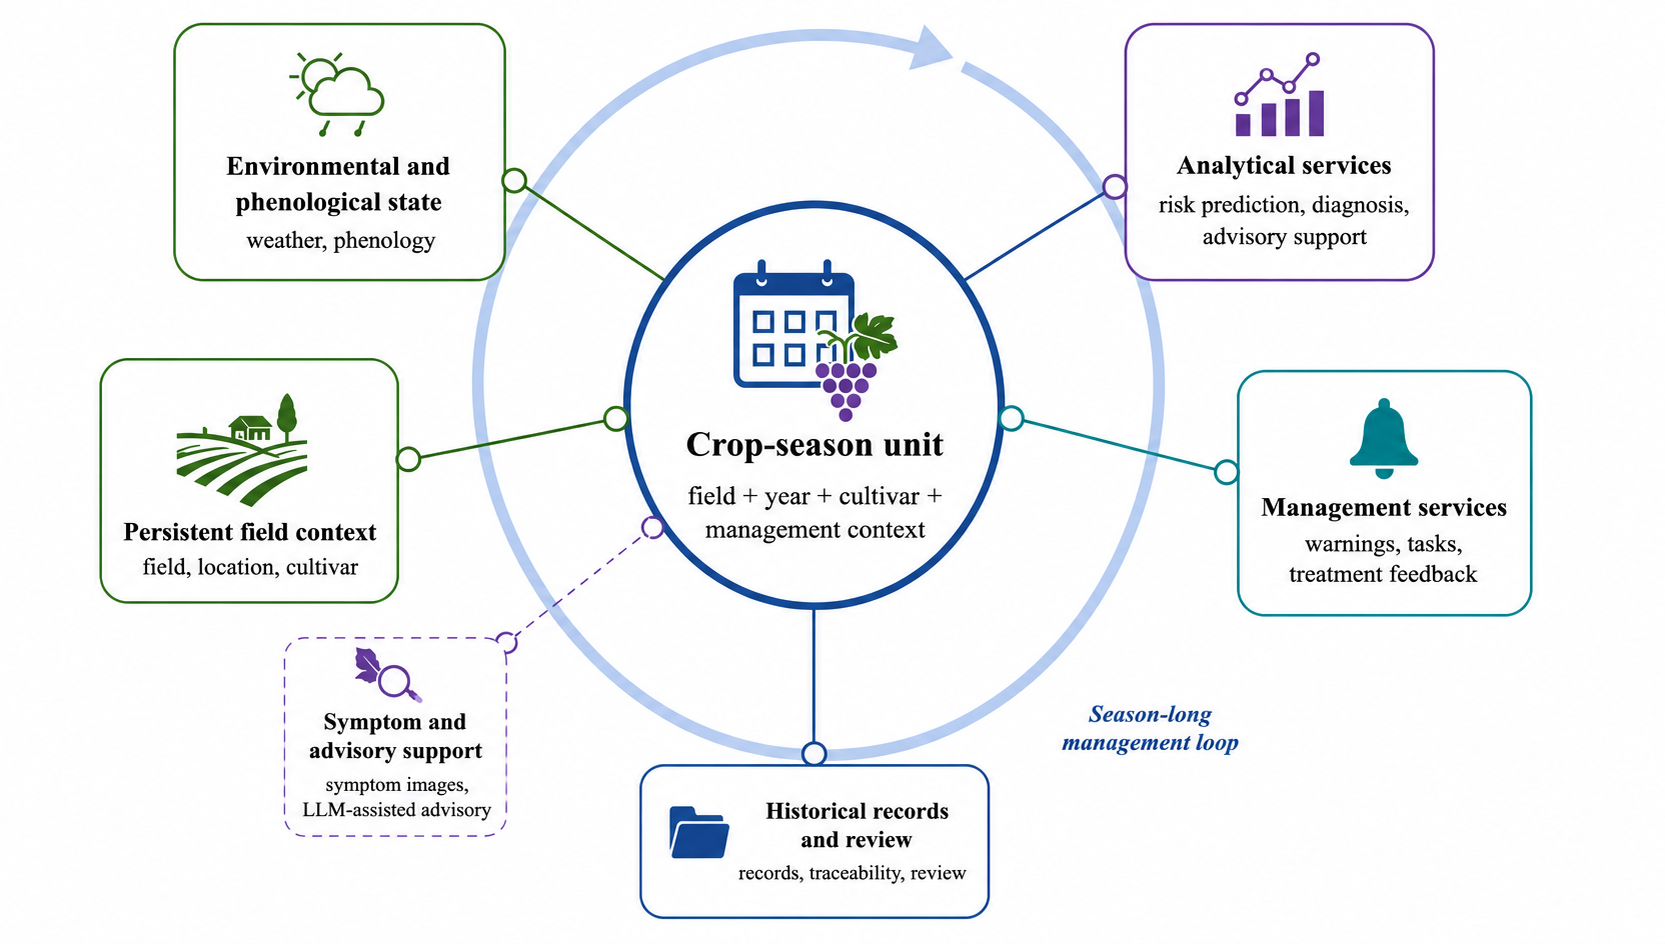
\includegraphics[width=\linewidth]{fig/figure1_new.png}
\caption[Crop-season-centered conceptual architecture]{Crop-season-centered conceptual architecture of GrapeMaster. The field and crop-season context coordinates environmental state, analytical services, management records, and post-symptomatic assistance. Arrows should be interpreted as software data or workflow relationships rather than proof that every record pair has a direct foreign key.}
\label{fig:crop_season_traceability_architecture}
\end{figure}

\subsection{Logical Architecture}\label{crop-season-object-and-workflow-states}

The logical architecture describes the records made available within one crop-season context. Shared crop, field, task, image, user, and message identifiers support retrieval at different strengths of linkage. For one crop-season context \(c\), the software-visible management state is represented as:
\begin{equation}
T_c =
\left(
F_c, M_c, W_c, P_c, R_c, N_c, O_c, B_c, E_c, A_c
\right),
\label{eq:crop_season_traceability_object}
\end{equation}
where \(F_c\) is the linked field record, \(M_c\) is crop metadata, \(W_c\) is weather input, \(P_c\) is phenology state, \(R_c\) is disease-risk output, \(N_c\) is event-delivery records, \(O_c\) is task or field-operation records, \(B_c\) is treatment-feedback records, \(E_c\) is symptom or image records, and \(A_c\) is advisory or message records. Weather, phenology, and disease results constitute analytical state; notifications and tasks constitute operational state; product records constitute management feedback; and images and advisory messages constitute the post-symptomatic branch. Table~\ref{tab:traceability_object} distinguishes their storage and retrieval roles.

The backend and mobile application implement a sequence of business operations around these objects. Weather and phenology updates prepare disease-model input; model responses supply risk states and treatment windows; notifications present events to users; tasks retain planned and completed operations; and fungicide products linked to tasks are converted into management-history input for applicable subsequent disease-service calls. A notification and a task can occur in the same crop context, but the current schema does not store a dedicated source-notification foreign key on the task. The software therefore supports a functional risk-to-action pathway and direct task-to-product feedback, while causal event-to-task provenance is not inferred. Table~\ref{tab:state_transition_rules} summarizes these transitions and linkage strengths.

\begin{table}[H]
\centering
\caption{Crop-season traceability object used in the GrapeMaster data architecture.}
\label{tab:traceability_object}
\tablefontsize
\begin{tabular}{@{}p{0.20\linewidth} p{0.36\linewidth} p{0.34\linewidth}@{}}
\toprule
Object element & Included records or payloads & Traceability function \\
\midrule
Crop context & Crop identifier, linked field identifier, cultivar, cultivation method, vine age, field coordinates, field size, and record timestamps & Defines the field-linked management context used by monitoring and operation resources; annual boundaries are an application convention rather than explicit schema fields \\
Environmental state & Weather records, historical and forecast weather payloads, and transformed hourly or daily weather inputs & Preserves the environmental exposure used by phenology, disease-risk, and operation-suitability services \\
Phenological state & Phenology payloads, broad phenological-stage labels, BBCH-related stage information, and stage descriptions & Links phenological-stage information to susceptibility interpretation, advisory timing, and task-related records \\
Disease-risk state & Disease-risk payloads, request-response bodies, field-risk states, protection states, treatment windows, and action recommendations & Connects model inputs, model outputs, and user-facing disease-risk interpretation under the same seasonal anchor \\
Operation state & Notification records, plant-protection tasks, irrigation tasks, task status, execution date, and overdue state & Stores event and field-operation records under the crop-season context \\
Treatment feedback & Fungicide or pesticide records linked to plant-protection tasks, product information, dosage information, and application date & Stores product-level management feedback for later protection-state interpretation and risk recalculation \\
Symptom and advisory records & Image-analysis records, advisory records, disease reports, field notes, and forum records where linked to account, field, crop season, or image identifiers & Preserves symptom-related records and advisory interaction for later management review \\
Review archive & Shared crop-season keys, task keys, payload availability, linkage checks, explicit absence notes for symptom records when absent, and review summaries & Supports management review of retained seasonal records \\
\bottomrule
\end{tabular}
\end{table}

\begin{table}[H]
\centering
\caption{Workflow state-transition rules used to define the crop-season management loop.}
\label{tab:state_transition_rules}
\tablefontsize
\begin{tabular}{@{}p{0.25\linewidth} p{0.35\linewidth} p{0.32\linewidth}@{}}
\toprule
State transition & Trigger or record basis & Platform interpretation \\
\midrule
Field setup to crop-season setup & A field record is created and a crop-season record is attached to that field & Establishes the seasonal management object \\
Crop-season setup to state updating & Weather and phenology payloads are generated or attached to the crop season & Provides environmental and phenological state for disease-risk interpretation \\
State updating to disease-risk interpretation & Disease-risk request-response payloads are attached to the same crop season & Converts weather, phenology, and management inputs into date-aligned disease-risk states \\
Disease-risk interpretation to event delivery & Warning or management notifications are generated under the retained account or crop-season context & Documents that analytical state was translated into user-facing events \\
Event delivery to task context & A plant-protection or irrigation task is created within the same user, field, or crop context & Converts a warning or management context into an executable operation record; a direct source-notification key is not stored \\
Task completion to treatment feedback & Completed plant-protection tasks are linked to fungicide or pesticide product records & Converts field operations into product-level management feedback \\
Treatment feedback to renewed disease-risk interpretation & Task serializers translate applicable product and execution records into recent fungicide-history input and invoke risk recalculation in supported pathways & Allows later disease-risk states to be interpreted in light of recorded management history \\
Workflow replay & Shared crop-season and task identifiers retrieve the sequence of state updating, disease-risk interpretation, event delivery, task execution, treatment feedback, and symptom/advisory branch availability & Reconstructs the management chain for workflow audit and management review \\
\bottomrule
\end{tabular}
\end{table}

\subsection{Service Architecture}\label{service-architecture}

The deployed software is organized into four service layers (Table~\ref{tab:architecture_layers}). The Flutter mobile layer manages interaction and presentation. The Django backend provides REST resources, authentication, identifier assignment, scheduled work, and business orchestration. Analytical processing is divided between backend processing and independently callable model services. PostgreSQL and JSON payload records provide persistence, while external weather, geocoding, messaging, classification, and advisory endpoints provide infrastructure or analytical functions not implemented in the mobile client.

\begin{table}[H]
\centering
\caption{Service architecture layers of GrapeMaster.}
\label{tab:architecture_layers}
\tablefontsize
\begin{tabular}{@{}p{0.22\linewidth} p{0.38\linewidth} p{0.34\linewidth}@{}}
\toprule
Layer & Main components & Main responsibilities \\
\midrule
Mobile application & Flutter interfaces and controllers for authentication, fields, crops, weather, risk, notifications, tasks, products, images, advisory chat, maps, and reports & Captures user input, presents backend resources, invokes post-symptomatic services, and supports field operations \\
Application backend & Django 4.2, Django REST Framework, JWT authentication, APScheduler, Channels, master-data tables, and business serializers & Owns REST resources, identifiers, scheduled updates, business rules, request construction, persistent records, and task-to-treatment translation \\
Analytical services & Weather and phenology processing, FastAPI disease service, spray-suitability calculation, hosted image classification, and streamed advisory endpoint & Converts environmental, crop, image, and text inputs into model outputs used by mobile functions \\
Persistence and external infrastructure & PostgreSQL, stored JSON request--response payloads, Agromodel weather/geocoding service, notification and SMS infrastructure, and hosted diagnostic/advisory services & Retains operational state and supplies external data or computations through network interfaces \\
\bottomrule
\end{tabular}
\end{table}

\section{Analytical-model integration}\label{analytical-model-integration}

This section explains how GrapeMaster integrates analytical components into software functions. The common pattern is: (1) identify the field and crop context; (2) assemble or receive a service-specific request; (3) invoke backend processing or a network service; (4) transform the response into a mobile-facing resource; and (5) retain the applicable input, output, or business record. Figure~\ref{fig:implementation_overview} summarizes this division of responsibility. The mobile client does not execute weather, phenology, or disease algorithms locally. Instead, it retrieves crop-keyed resources from the backend. Image classification and advisory interaction form a second path in which the mobile client calls separately hosted endpoints.

\begin{figure}[H]
\centering
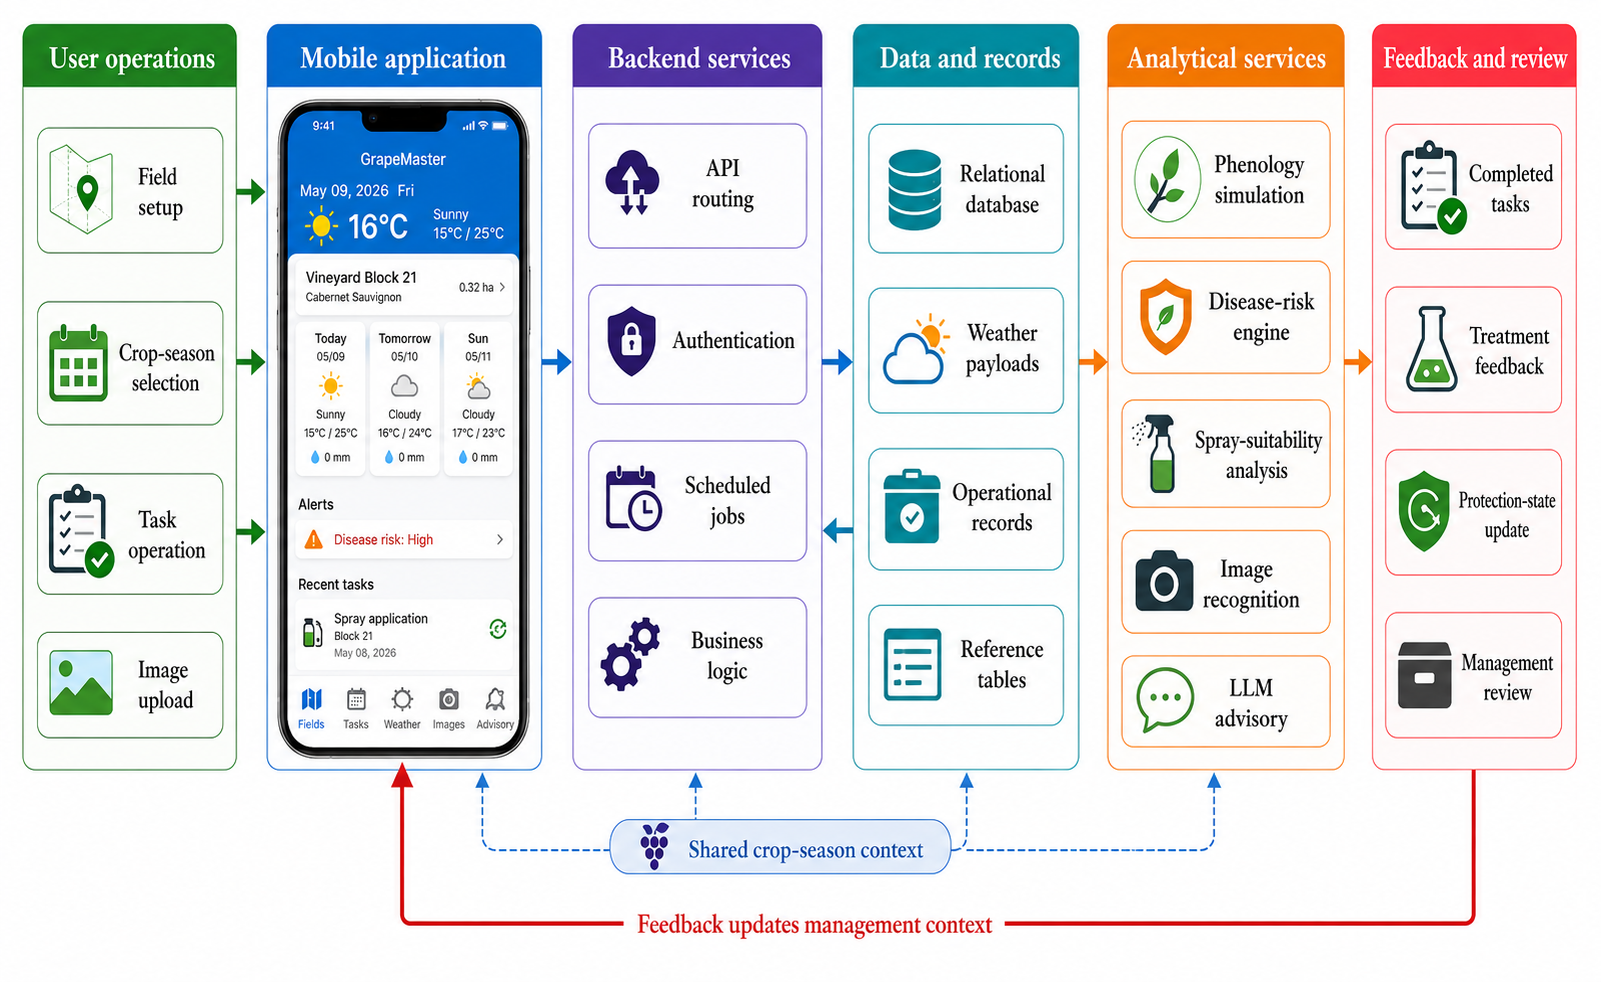
\includegraphics[width=\linewidth]{fig/figure3_new.png}
\caption[Mobile--backend implementation flow]{Mobile--backend implementation flow of GrapeMaster under a shared crop-season context. The Django backend owns the principal management records and orchestrates environmental and disease processing; the post-symptomatic image and advisory services are separately hosted.}
\label{fig:implementation_overview}
\end{figure}

\begin{table}[H]
\centering
\caption[Analytical-service integration in GrapeMaster]{Analytical-service inputs, invocation patterns, outputs, and software roles in GrapeMaster.}
\label{tab:module_provenance}
\tablefontsize
\begin{tabular}{@{}p{0.16\linewidth} p{0.25\linewidth} p{0.22\linewidth} p{0.27\linewidth}@{}}
\toprule
Service & Principal inputs & Invocation and retained output & User-facing role \\
\midrule
Weather and spray suitability & Field coordinates and requested time window & Scheduled and on-demand backend calls to Agromodel; crop-linked weather JSON and transformed hourly/daily series & Weather forecast, historical conditions, and operation-suitability display \\
Phenology & Daily temperature, cultivar, and crop metadata & Backend processing during scheduled crop refresh; crop-linked phenology payload and daily stage sequence & Host-development display and susceptibility context \\
Disease risk & Hourly weather, daily growth stage, susceptibility, disease target, and applied-fungicide history & Stateless FastAPI request; backend stores request/response and derived disease summary under the crop identifier & Risk timeline, field-risk state, treatment windows, and warning content \\
Image recognition & User-selected grape symptom image & Hosted HTTP classification call; classification text and confidence presented to the client and retained where the service contract permits & Post-symptomatic disease or healthy-category assistance \\
LLM advisory & User question and available diagnostic context & Hosted WebSocket interaction streams text until an end marker; advisory/message records are available through application services & Follow-up explanation and management-oriented consultation \\
\bottomrule
\end{tabular}
\end{table}

\subsection{Weather and phenology processing}\label{weather-and-phenology-processing}

Weather processing uses field coordinates and crop identifiers to retrieve historical observations and a 16-day forecast from the Agromodel weather service. Crop creation initializes the weather resource, and a backend scheduler refreshes active crop records each morning. During a refresh, the backend obtains weather, prepares daily values for phenology, prepares hourly values for the disease service, calculates spray-suitability information, and stores aggregate weather, phenology, disease-response, and disease-request payloads. A retry pass handles crops that fail during the first weather-fetch cycle. The weather provider named here reflects the backend version documented in this paper; a different provider should be reported only if a versioned deployment artifact establishes that configuration.

Phenology processing receives daily temperature together with cultivar and crop metadata. It produces a crop-linked payload for mobile display and a date-aligned growth-stage sequence for the disease request. The integration therefore uses phenology twice: as a visible description of crop development and as host-state input for interpreting disease susceptibility. The reported Guangxi broad-stage validation in Section~\ref{supporting-analytical-components} characterizes the platform-compatible phenology configuration rather than a new phenology algorithm proposed by this paper.

\subsection{Disease-risk service}\label{disease-risk-service-and-treatment-feedback-workflow}

The disease service is exposed through FastAPI and is stateless between requests. The Django backend assembles the complete calculation context: hourly weather, a daily growth-stage sequence, cultivar susceptibility, target-disease settings, and recent fungicide history. The service validates the request, executes the applicable disease pipeline, and returns date-aligned infection or disease states, field-risk interpretation, protection state, recommendations, and treatment windows. The current service source contains active grape downy mildew and powdery mildew pathways. The mobile client does not call this service directly; it retrieves the persisted disease summary from crop-keyed Django resources.

The backend stores both the request and response in crop-linked records. This is important because the disease service itself has no database and the current Django integration does not transmit the actual crop UUID in the service's optional \texttt{crop\_season\_uuid} field. Traceability is therefore supplied by the backend association between the crop resource and its retained payloads, not by the disease service. Figure~\ref{fig:disease_risk_engine_structure} shows the integration sequence.

\begin{figure}[H]
\centering
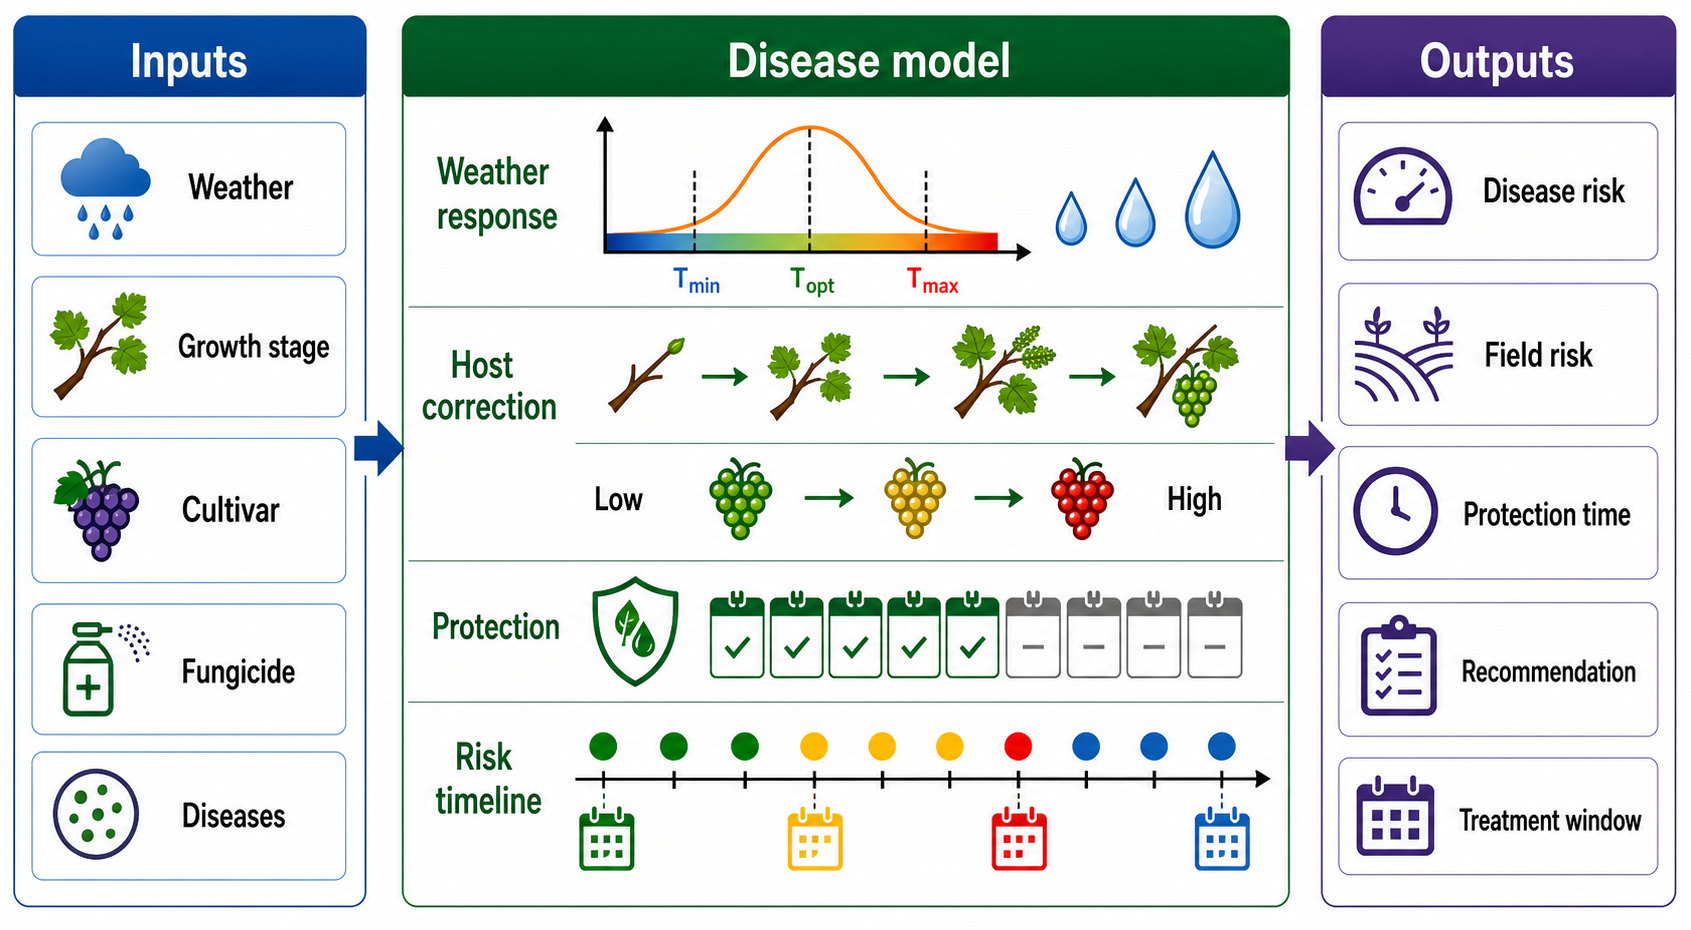
\includegraphics[width=\linewidth]{fig/fig03_disease_model_workflow.png}
\caption[Disease-service integration workflow]{Disease-service integration workflow in GrapeMaster. The backend prepares environmental, phenological, susceptibility, disease-target, and management inputs; the stateless service returns date-aligned disease and field-risk information; and the backend retains request and response payloads for mobile delivery and later updating.}
\label{fig:disease_risk_engine_structure}
\end{figure}

The Guangxi first-infection result reported later was produced for the team-developed FSIM-S configuration. It demonstrates the suitability of one downy mildew component for the platform interface. Because the available runtime snapshot does not contain an immutable identifier linking every deployment response to that evaluated configuration, the paper treats the result as supporting component evidence rather than as proof of the exact model version used for every historical record.

\subsection{Treatment feedback and recalculation}\label{treatment-feedback-and-recalculation}

Plant-protection tasks and their product records provide the most direct connection between analytical and management services. A fungicide or pesticide product has a direct task relationship. When an applicable task is stored or completed, backend serializers translate target disease, execution date, and protection-duration information into the \texttt{applied\_fungicides} structure expected by the disease service. The stored disease request is updated and the disease service is invoked asynchronously in supported task pathways. This produces a revised response in which recent management history can affect the interpreted protection state and recommendations.

The active disease-service implementation relies principally on disease target, application date, and configured protection durations; efficacy fields accepted by the request schema are not fully used by the current calculation. Accordingly, the manuscript describes treatment-aware recalculation rather than individualized chemical-efficacy simulation. This boundary is consistent with the temporary nature of fungicide protection under host growth, rainfall, and disease pressure \citep{caffiFungicideModelsAre2018,oliverFungicideUsePatterns2023,warnekeEffectFungicideMobility2020}.

\subsection{Image-recognition and advisory services}\label{image-recognition-and-advisory-services}

The post-symptomatic workflow begins when a user photographs or selects a grape image. The Flutter client submits the image to a separately hosted classification service, parses the returned classification text, and displays the category and associated explanation. The result can be reported against a selected field. A severity function is also available through a separate hosted endpoint. These services are external to the principal Django deployment and must preserve the response contracts expected by the client.

After classification, the advisory interface offers follow-up questions and sends user text to a hosted WebSocket service. Responses are streamed until an end marker is received. The software role of this component is interaction and explanation: it complements, but does not replace, the epidemiological disease service, expert diagnosis, pesticide labels, or regulated plant-protection decisions. The design follows the image-plus-ChatGLM3 concept reported for CDIP-ChatGLM3 \citep{yanCDIPChatGLM3DualmodelApproach2025}. The repository version documented for this paper establishes the client endpoint and message flow, but does not include the hosted model checkpoint, fine-tuning corpus, prompt, or deployment version. The present paper therefore claims integration of an LLM-assisted advisory interface and reports message records, but does not claim independent validation or full artifact-level reproducibility of the hosted LLM.

\begin{figure}[H]
\centering
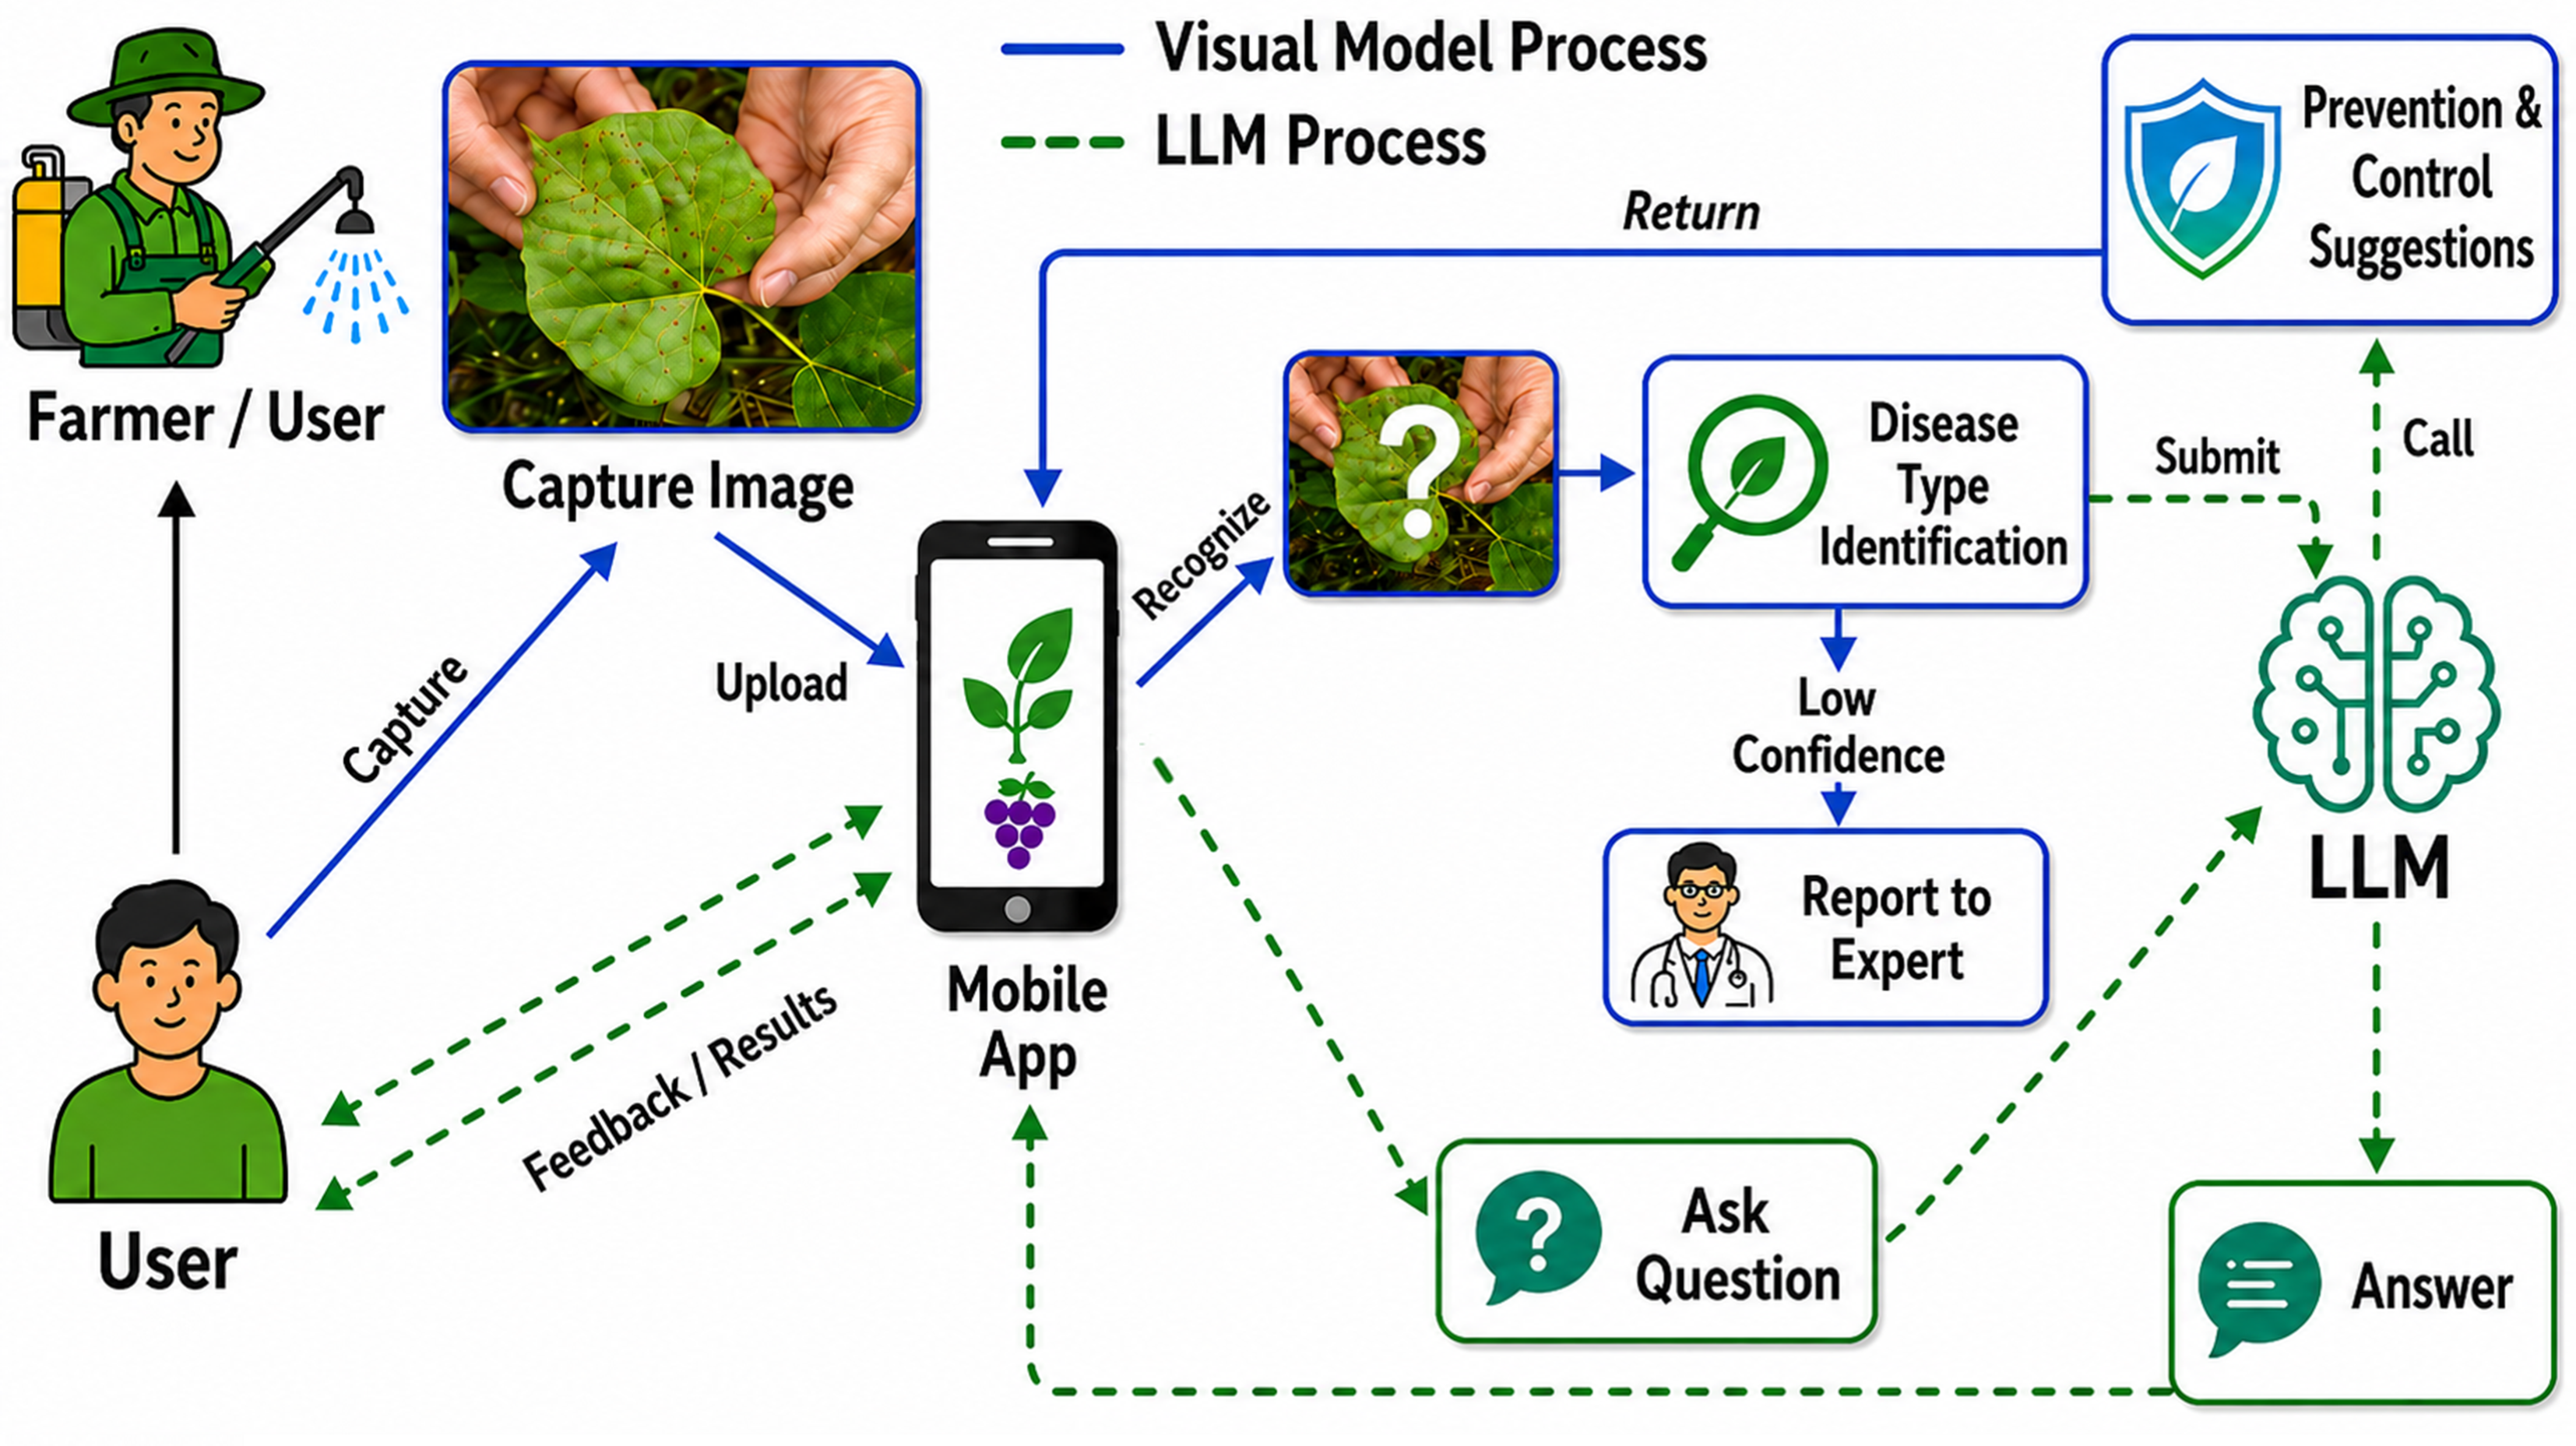
\includegraphics[width=\linewidth]{fig/fig13_image_assistance_workflow.png}
\caption[Image-recognition and advisory workflow]{Image-recognition and LLM-assisted advisory workflow in GrapeMaster. The mobile client invokes separately hosted image and advisory services, presents their responses, and can associate a diagnostic report with a field. LLM, large language model.}
\label{fig:image_advisory_workflow}
\end{figure}

\section{Software functions and operational workflows}\label{features-and-functionalities}

The architecture is presented to users through two principal workflows. The pre-symptomatic workflow connects field setup, weather and phenology monitoring, disease-risk display, notifications, tasks, product records, and treatment-aware review. The post-symptomatic workflow connects image capture, disease classification, streamed advisory interaction, and optional reporting. This section describes the functions as user workflows rather than as independent screens.

\subsection{Field configuration and crop-context monitoring}\label{field-and-crop-season-workspace}

The mobile application begins with authentication, a field list, and map-based field-boundary definition (Figure~\ref{fig:field_crop_season_entry_points}). Field creation transfers geometry and management information to the backend, which creates identifiers and derives or requests location information. A crop resource is then attached to the field using cultivar, cultivation method, and vine-age information. The crop workspace retrieves weather, phenology, and disease summaries through separate backend resources keyed by that crop UUID.

\begin{figure}[H]
\centering
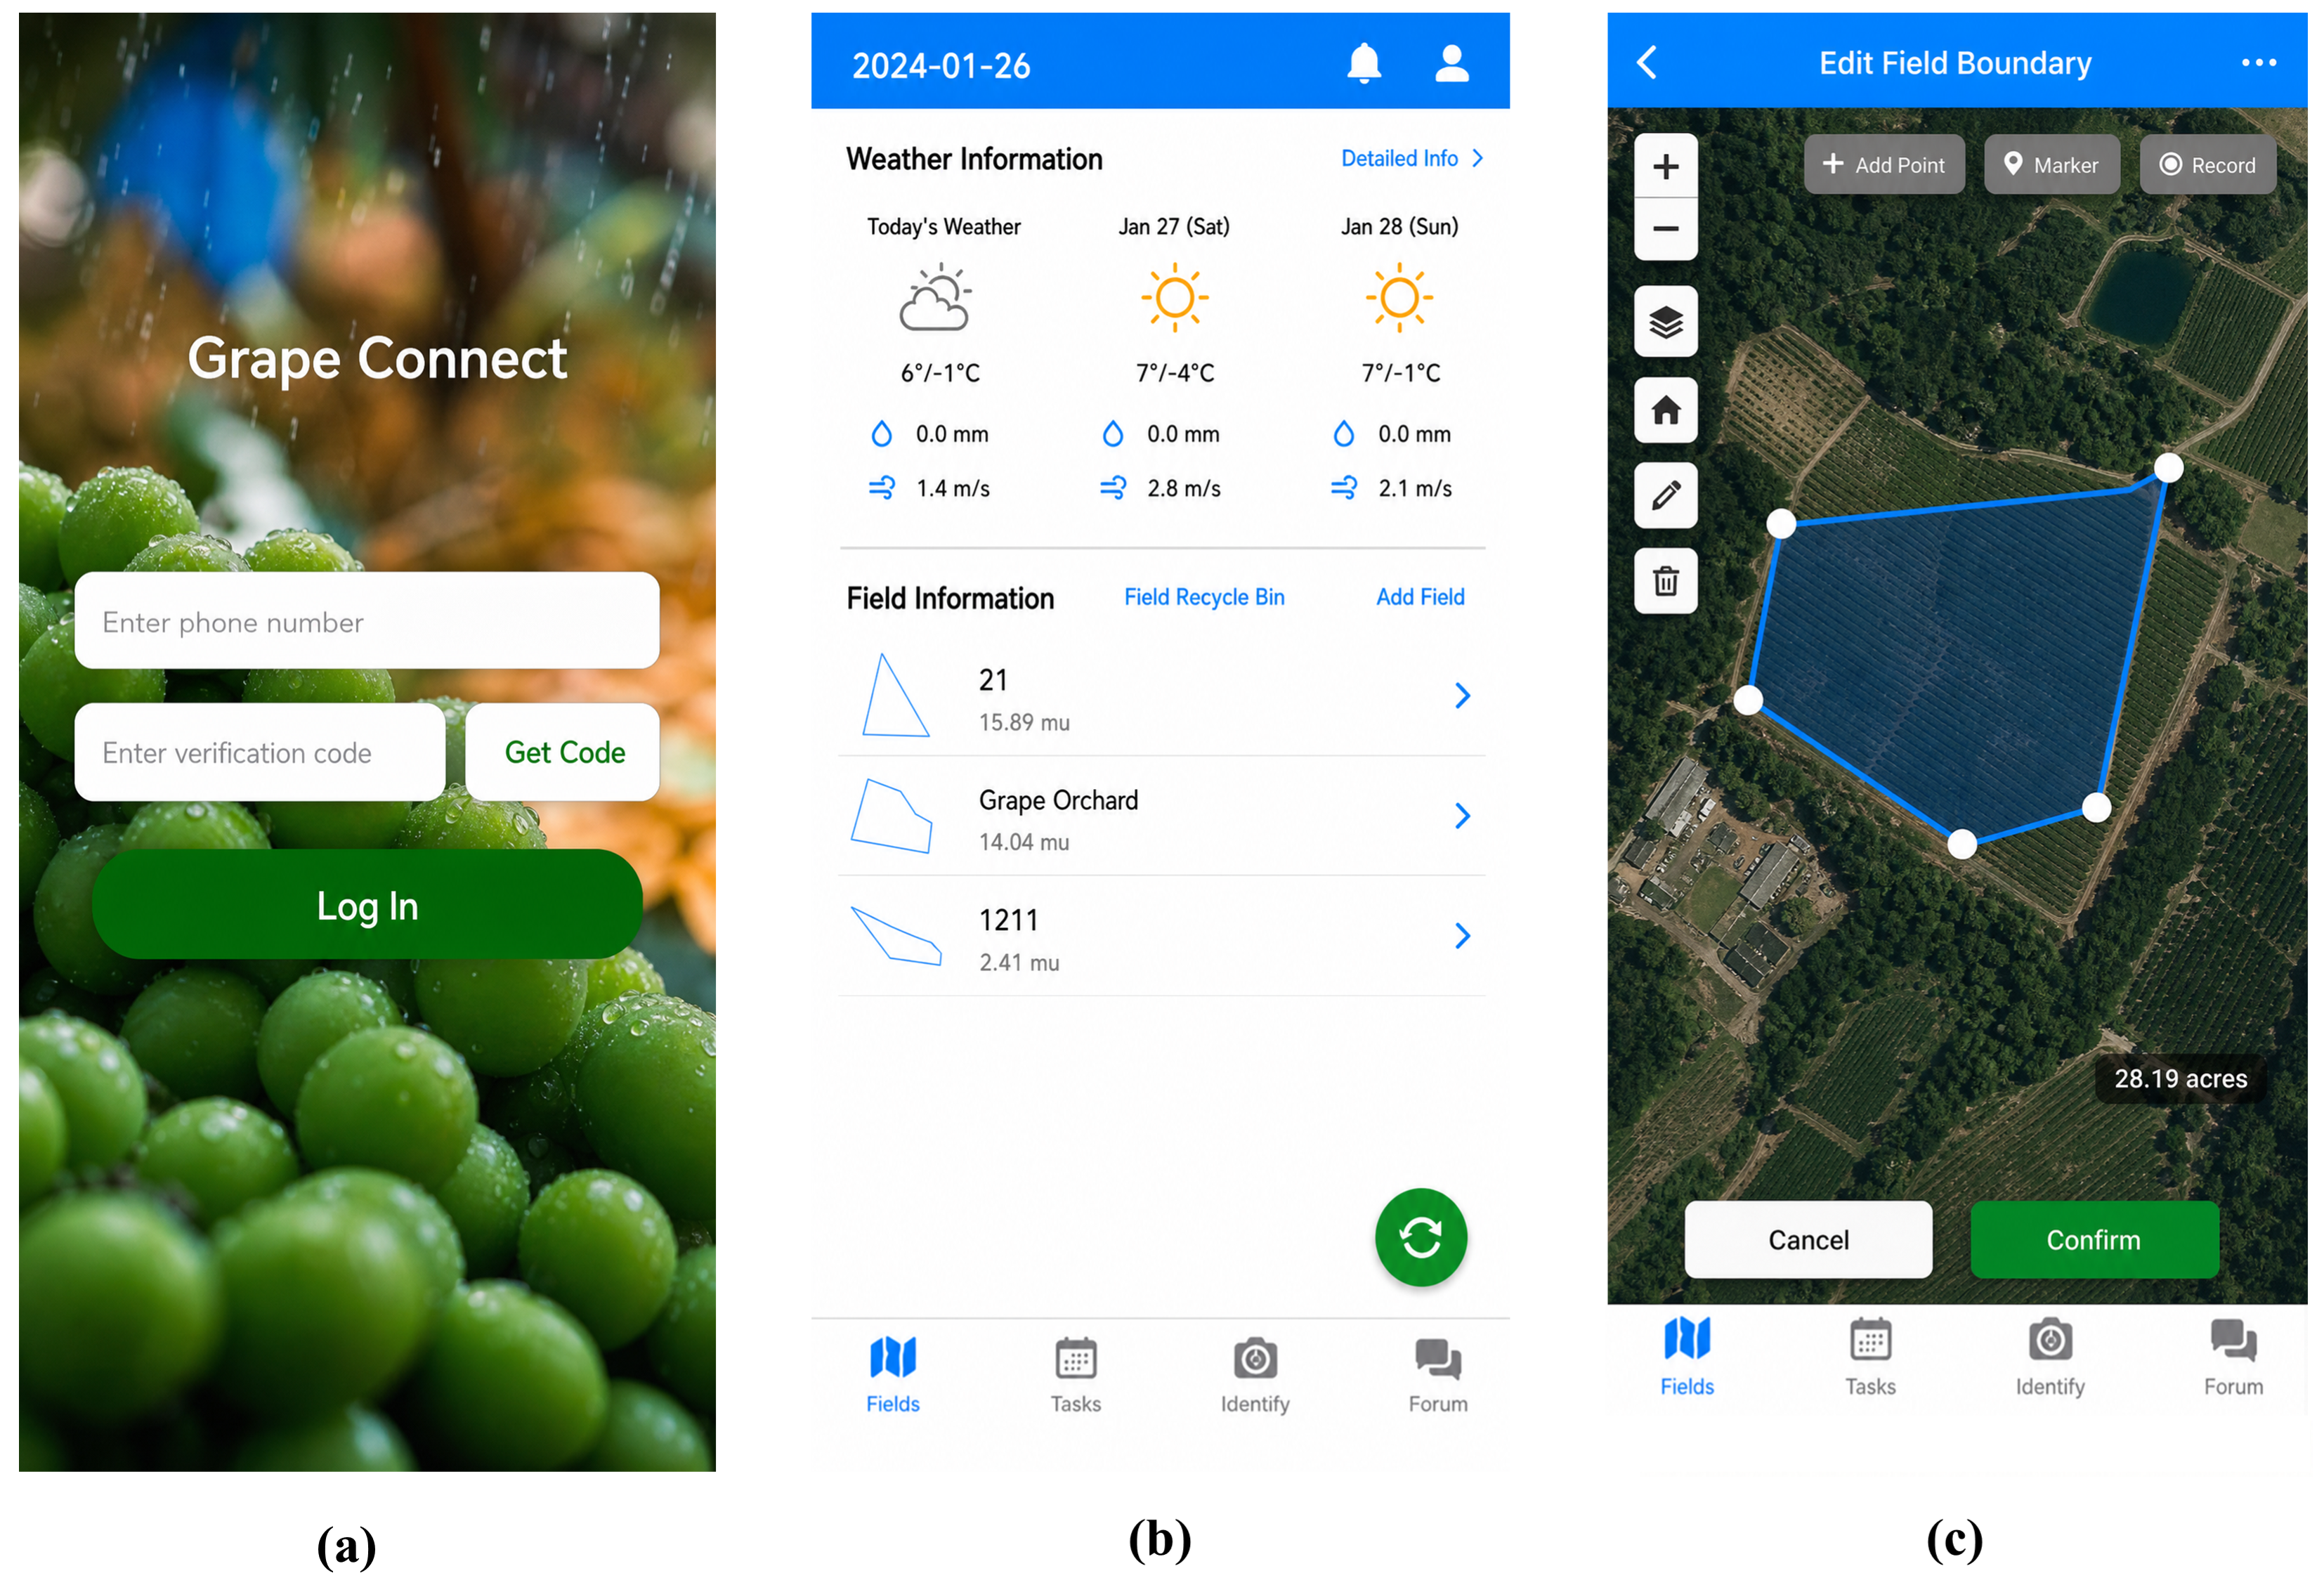
\includegraphics[width=\linewidth]{fig/field_management_interfaces.png}
\caption[Field and crop-context entry points]{Field and crop-context entry points in GrapeMaster: account access, vineyard selection, and map-based field-boundary editing.}
\label{fig:field_crop_season_entry_points}
\end{figure}

Within the selected context, GrapeMaster presents near-term weather, spray-suitability information, broad phenological stage, and field-level disease summaries (Figure~\ref{fig:weather_phenology_interfaces_result}). The mobile layer is primarily a workflow and presentation client for these prepared backend resources. This design keeps model dependencies out of the device while giving different analytical services a consistent field-oriented entry point.

\begin{figure}[H]
\centering
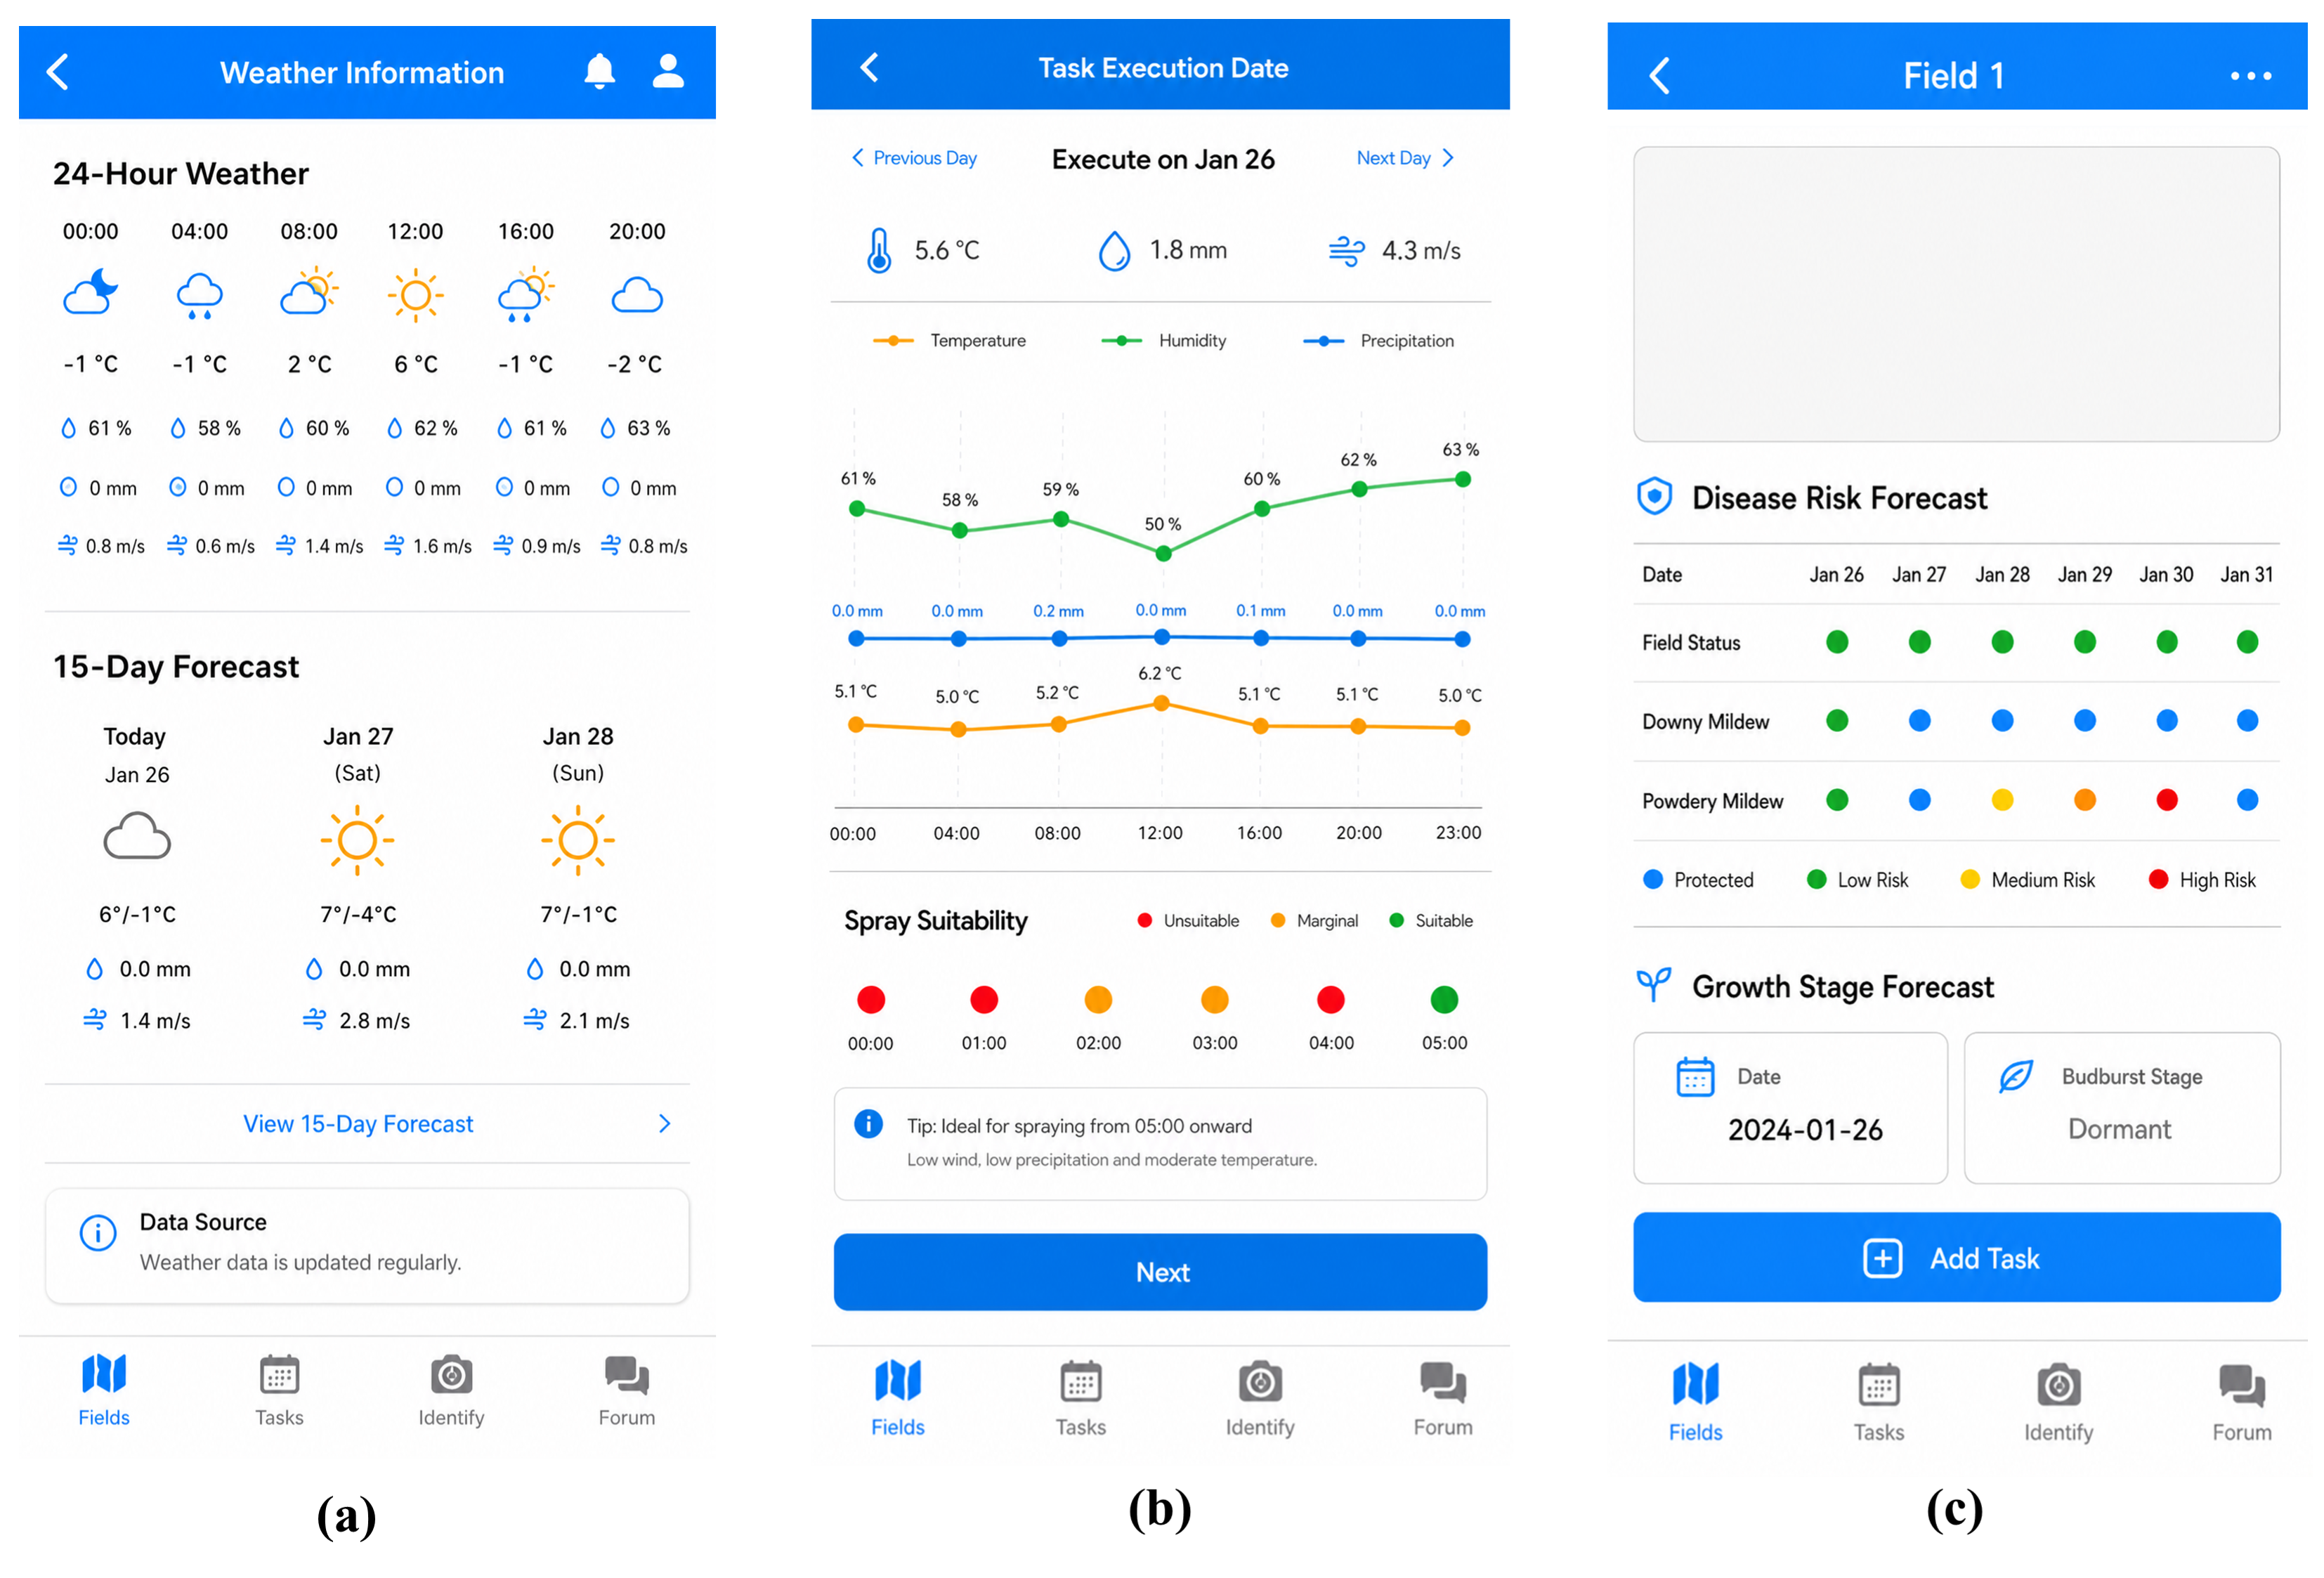
\includegraphics[width=\linewidth]{fig/weather_phenology_interfaces.png}
\caption[Crop-season workspace for weather and phenology state]{Crop-season workspace for weather and phenology state in GrapeMaster. (a) The weather page displays near-term field-specific weather information. (b) The spray-suitability page displays hourly weather and spray-suitability information. (c) The crop-season workspace displays field-risk and phenological-stage summaries under the selected field context.}
\label{fig:weather_phenology_interfaces_result}
\end{figure}

\subsection{Disease-risk workflow and treatment feedback}\label{risk-display-and-notification-delivery}\label{task-execution-and-product-feedback}

GrapeMaster organizes disease outputs into a risk-to-action-to-feedback workflow under the selected crop context. Date-aligned timelines present disease and field-risk states and can show protection-state changes after fungicide history is incorporated (Figure~\ref{fig:disease_risk_timeline_result}). The important software function is the continuity between model resources, reviewable events, executable task records, direct task-to-product relationships, and updated risk interpretation.

When a disease-risk or management event is generated, GrapeMaster delivers it as a reviewable alert or reminder and retains it in the notification archive (Figure~\ref{fig:alert_notification_interfaces_result}). Users can create a plant-protection task within the same management context. The task does not retain a direct source-notification identifier, so the relationship is functional and contextual rather than a database-level causal link. Task and product records retain operation status, timing, product, dosage, field area, water volume, and mixing information (Figure~\ref{fig:task_management_interfaces_result}). Product records are directly linked to their tasks and can become disease-service management input.

\begin{figure}[H]
\centering

\includegraphics[width=\linewidth]{fig/disease_risk_timeline_downy_field.png}
\caption[Disease-risk timeline and treatment-feedback update]{Disease-risk timeline and treatment-feedback update in GrapeMaster. (a) Mingyang 2024 shows date-aligned downy mildew and field-risk states. (b) A Guangxi crop-season case without fungicide feedback records shows the untreated disease-risk state sequence. (c) The same Guangxi crop-season case with fungicide feedback records shows the corresponding protected-state updates.}
\label{fig:disease_risk_timeline_result}
\end{figure}

\begin{figure}[H]
\centering
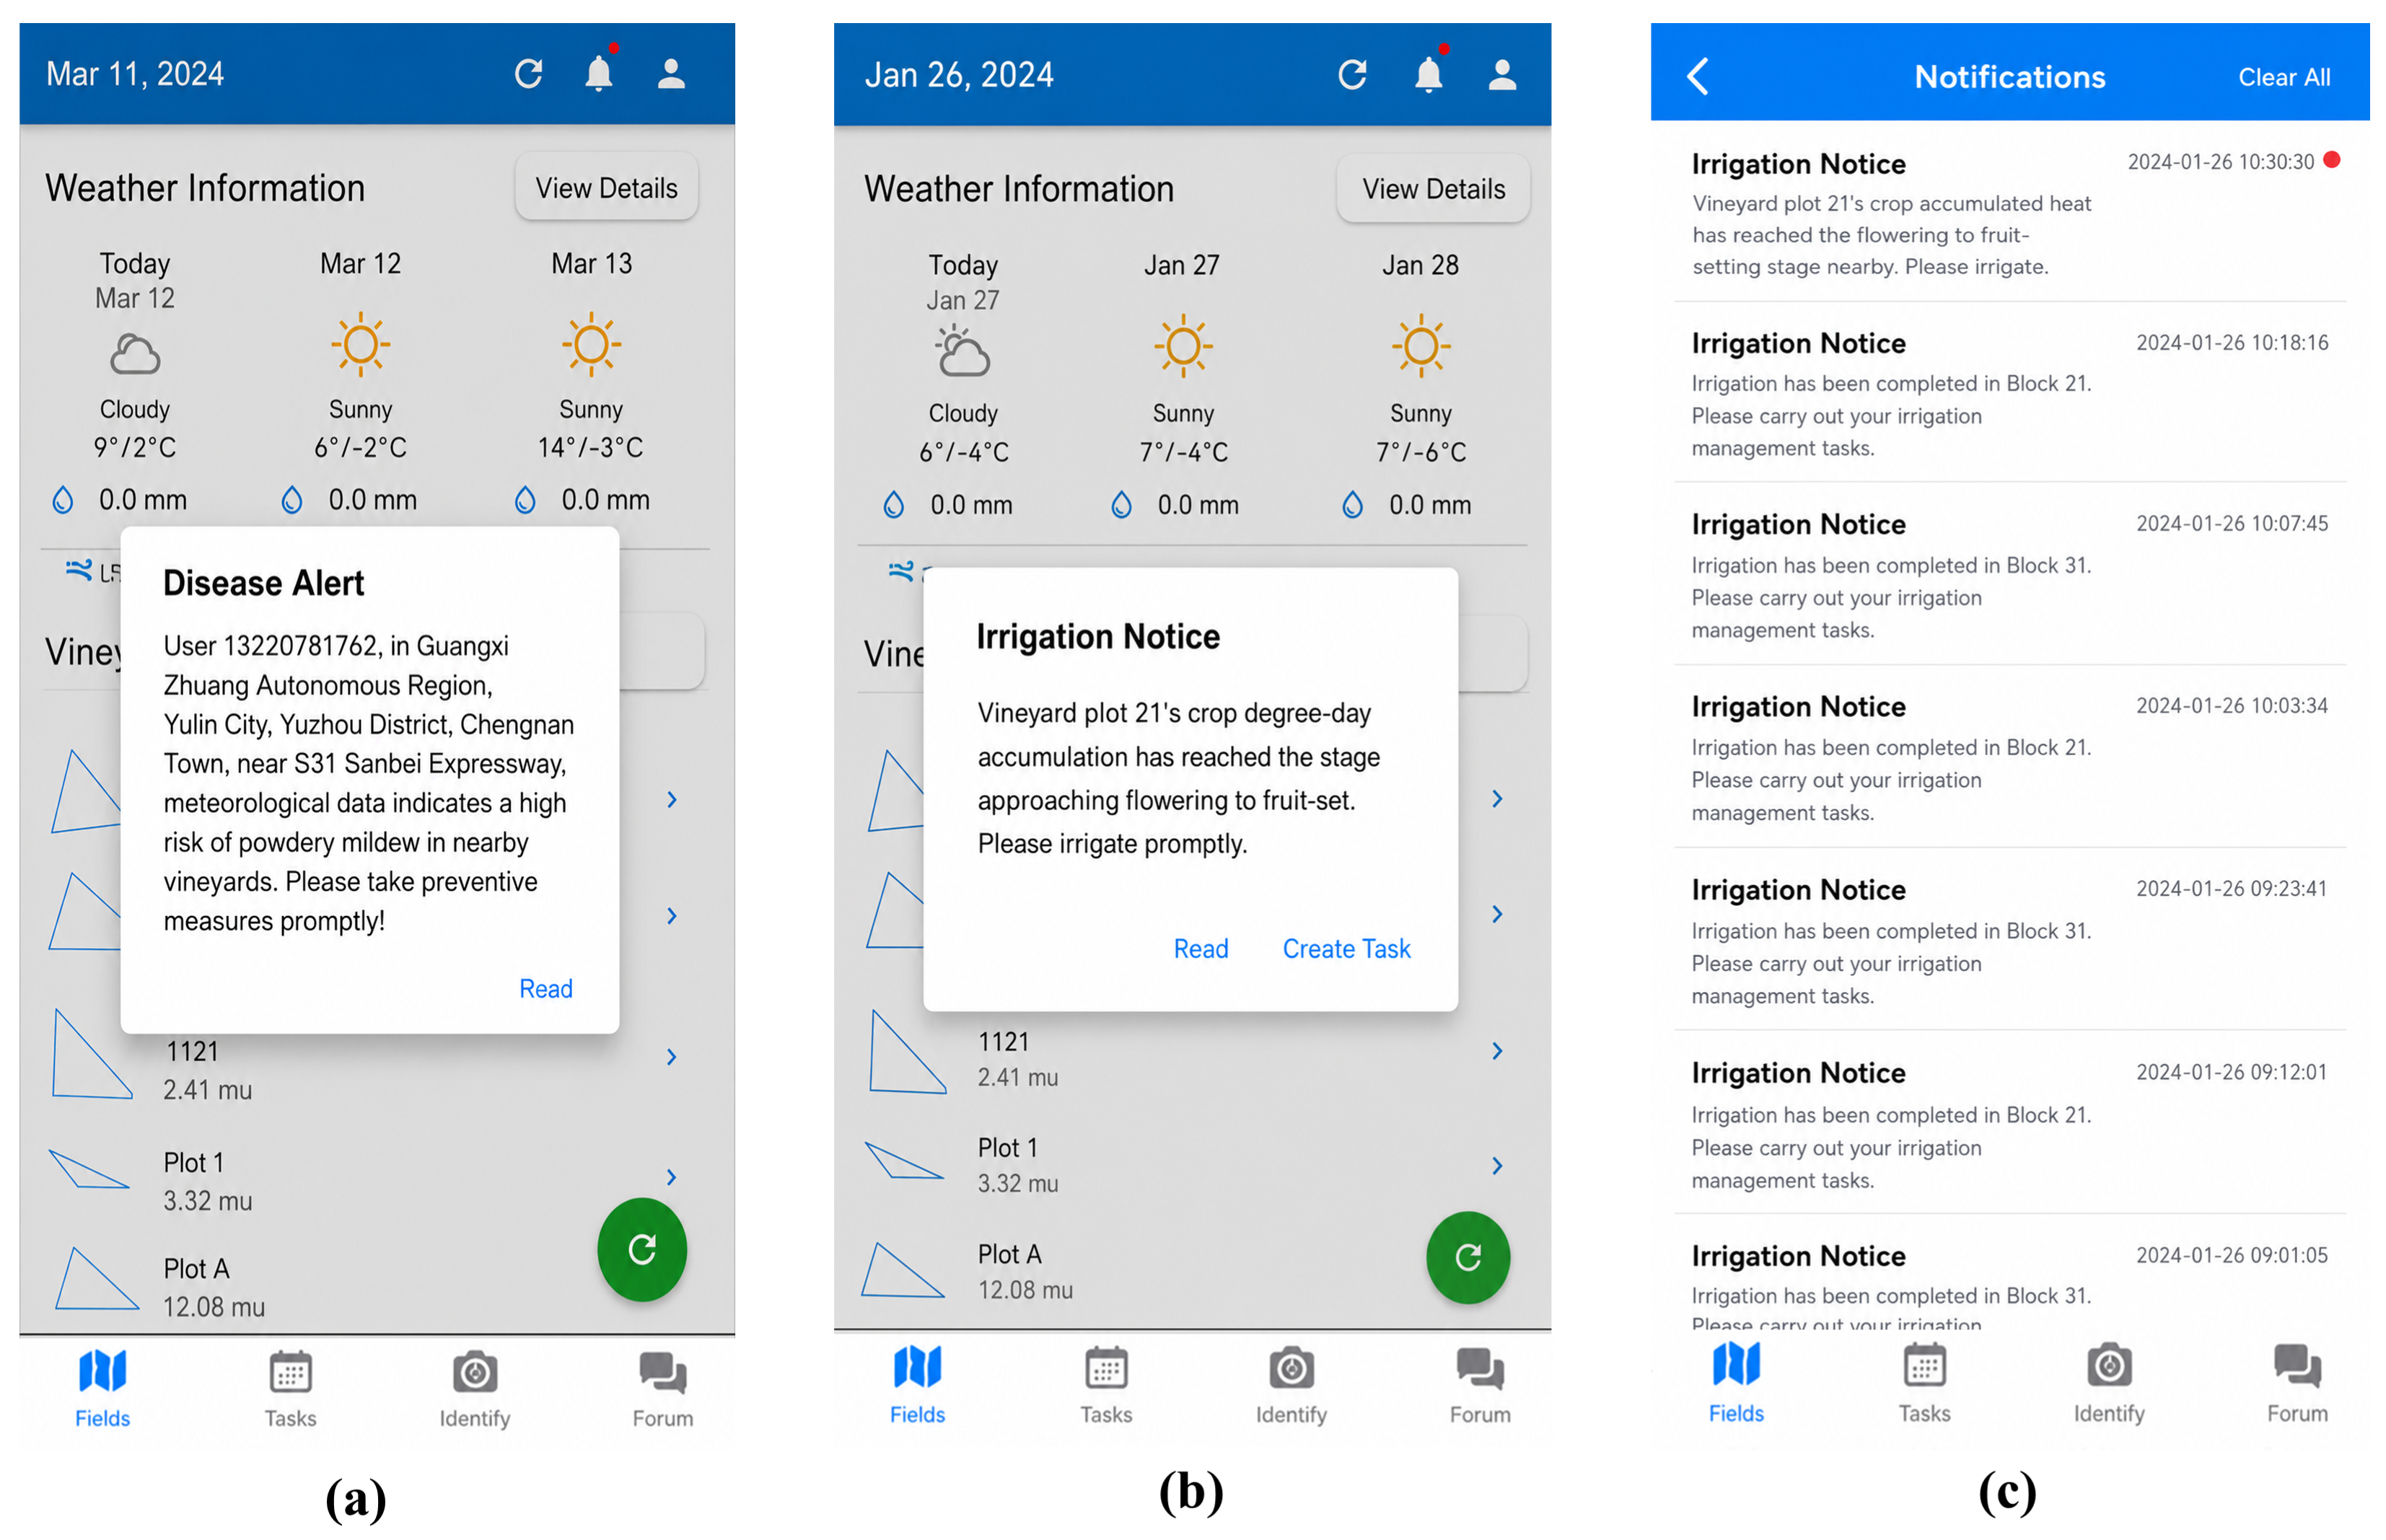
\includegraphics[width=\linewidth]{fig/alert_notification_interfaces.png}
\caption[Warning and notification records for crop-season events]{Warning and notification records for crop-season events in GrapeMaster. (a) The disease-alert dialog displays a crop-season disease-risk event. (b) The management notice dialog provides a task-related reminder. (c) The notification list archives reviewable crop-season events.}
\label{fig:alert_notification_interfaces_result}
\end{figure}

\begin{figure}[H]
\centering
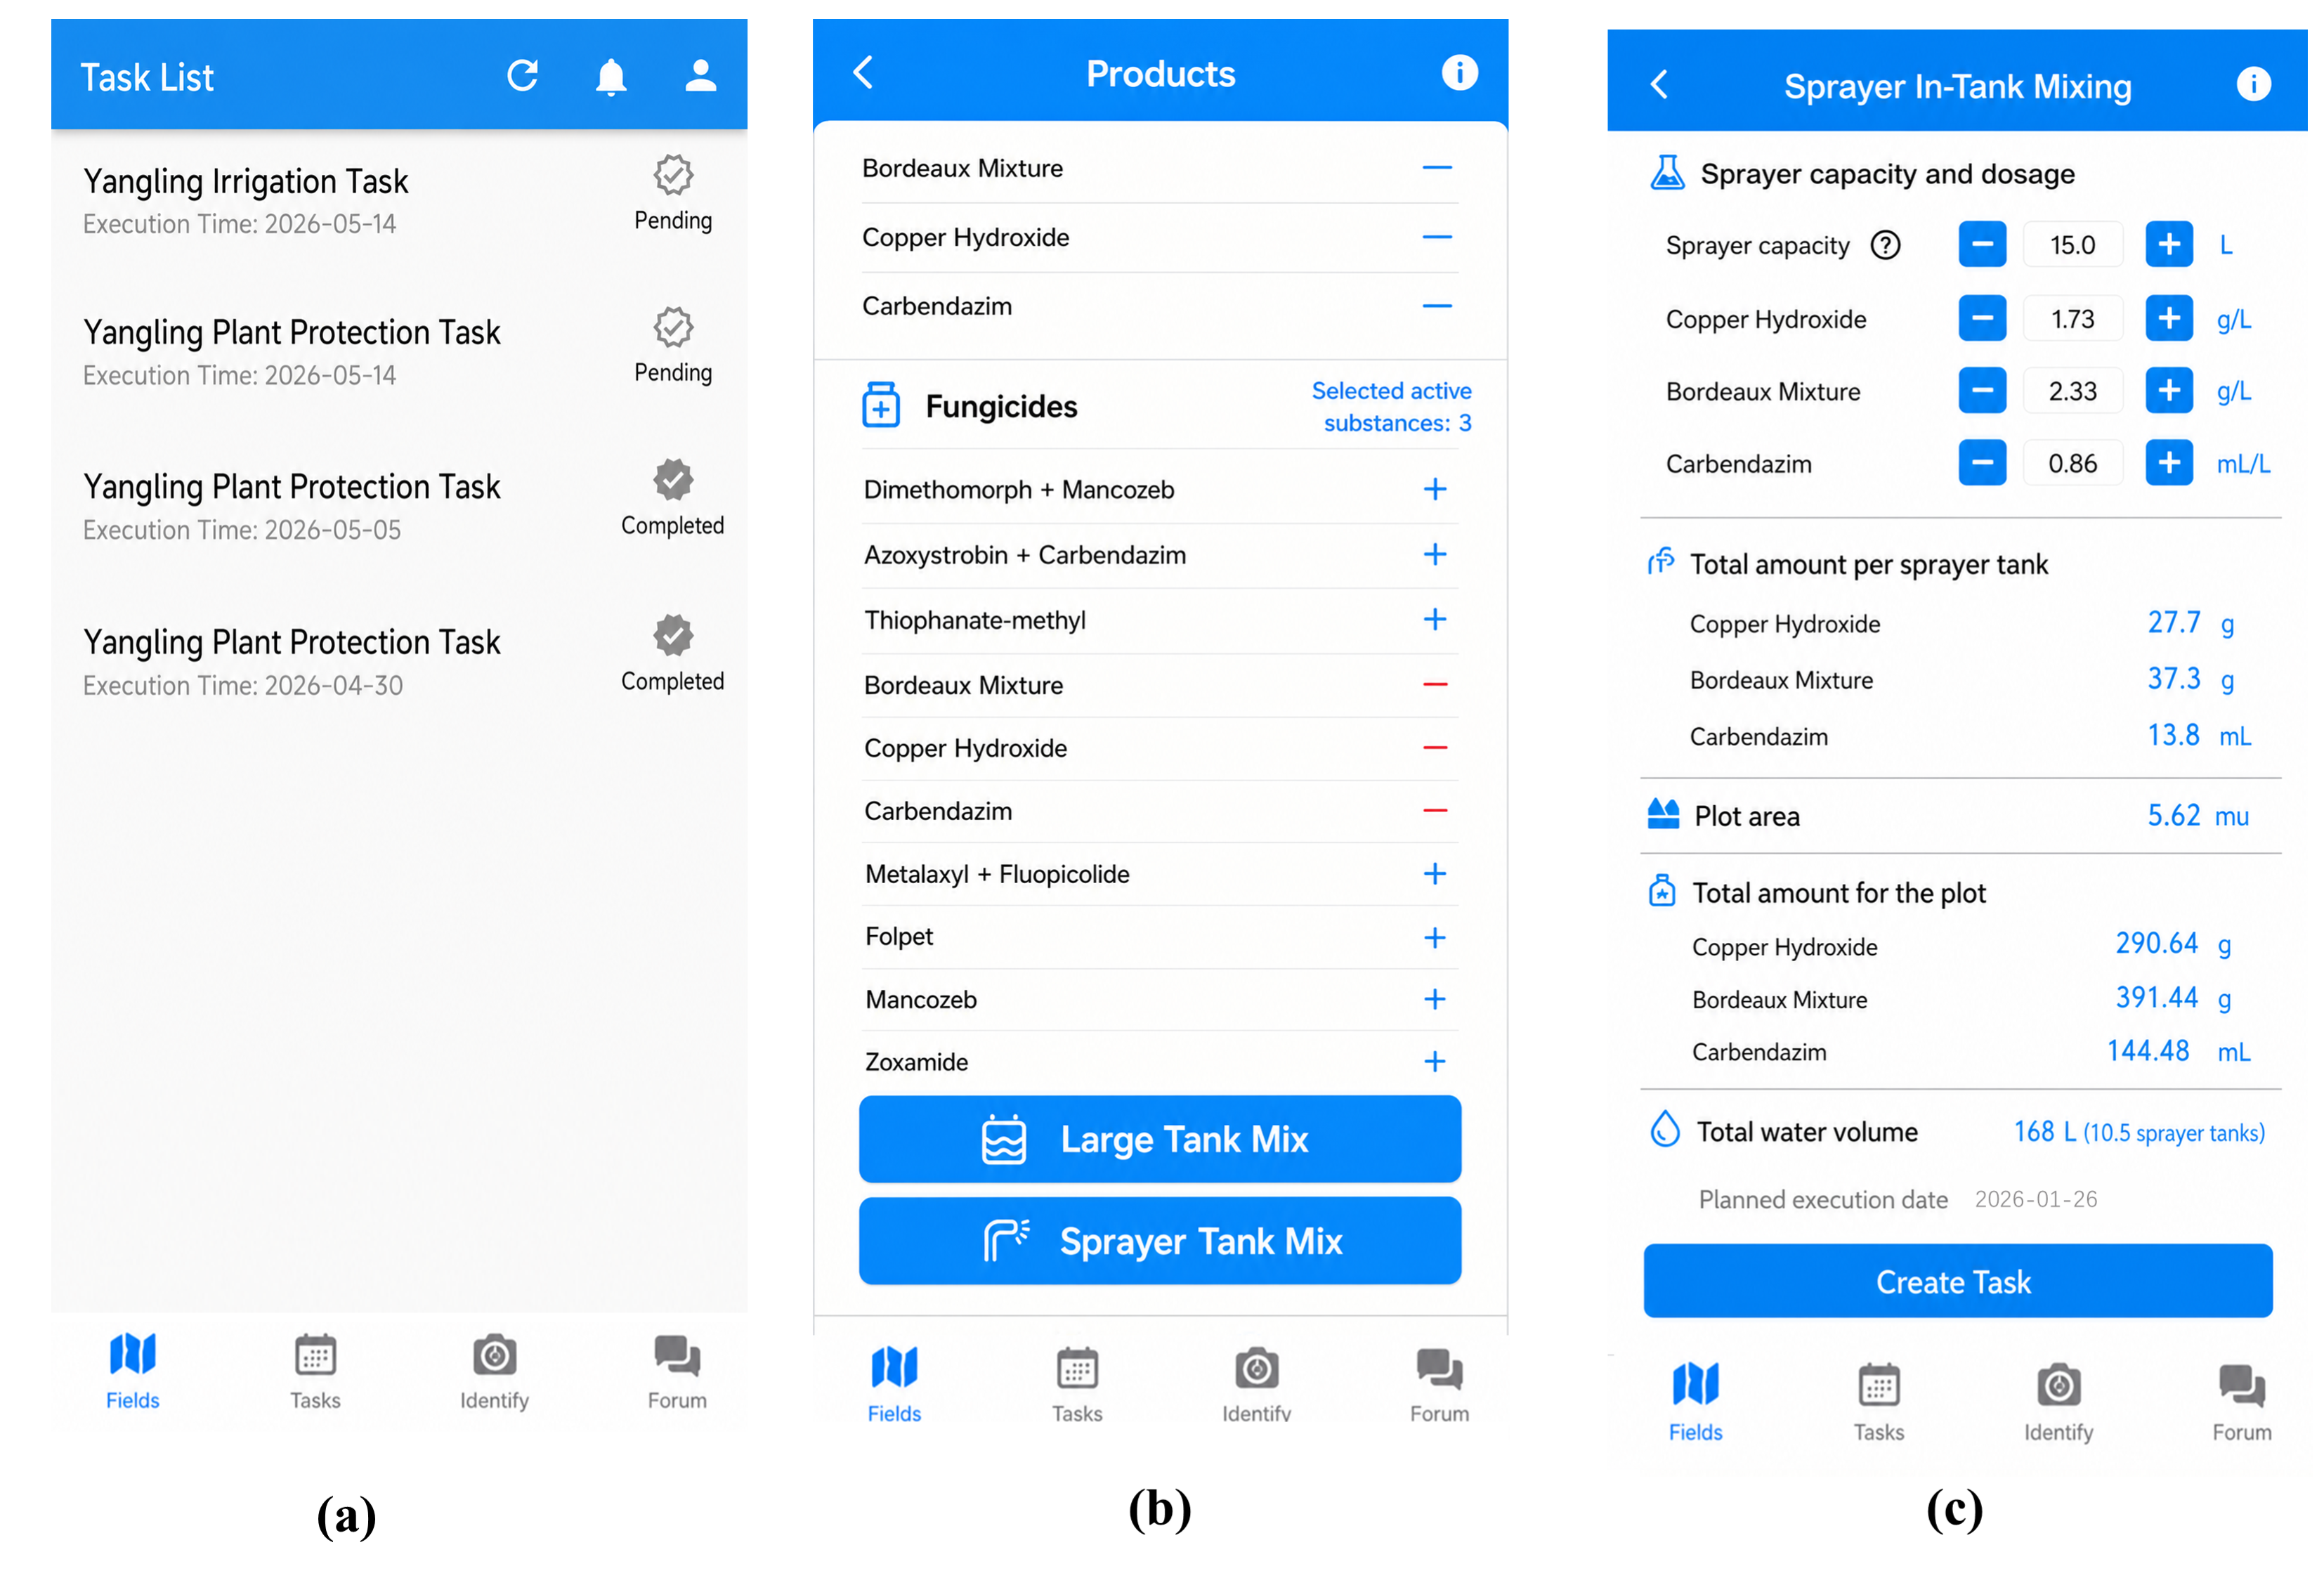
\includegraphics[width=\linewidth]{fig/task_management_interfaces.png}
\caption[Task creation and treatment-feedback interfaces]{Task creation and treatment-feedback interfaces in GrapeMaster. (a) The task list records field operations and task status. (b) The product selection page stores fungicide or pesticide entries linked to plant-protection tasks. (c) The in-tank mixing page records sprayer capacity, product dosage, plot area, water volume, and planned date.}
\label{fig:task_management_interfaces_result}
\end{figure}

\subsection{Symptom recognition and advisory support}\label{symptom-image-and-advisory-functions}

GrapeMaster provides a second workflow for post-symptom evidence and interactive assistance (Figure~\ref{fig:ai_diagnosis_interfaces_result}). After an image is uploaded, the hosted classifier returns disease or healthy-category text and confidence information. The result view exposes predefined follow-up questions, while the advisory WebSocket streams management-oriented text to the interface. Users can optionally report the interpreted diagnosis against a field. Image, report, advisory, and message records remain available in the wider application environment, although their identifiers vary: reports can reference fields, notes can reference crop records, and advisory messages are primarily user- or message-keyed. The paper therefore treats this branch as functionally integrated without asserting that every advisory exchange has a direct crop foreign key.

\begin{figure}[H]
\centering
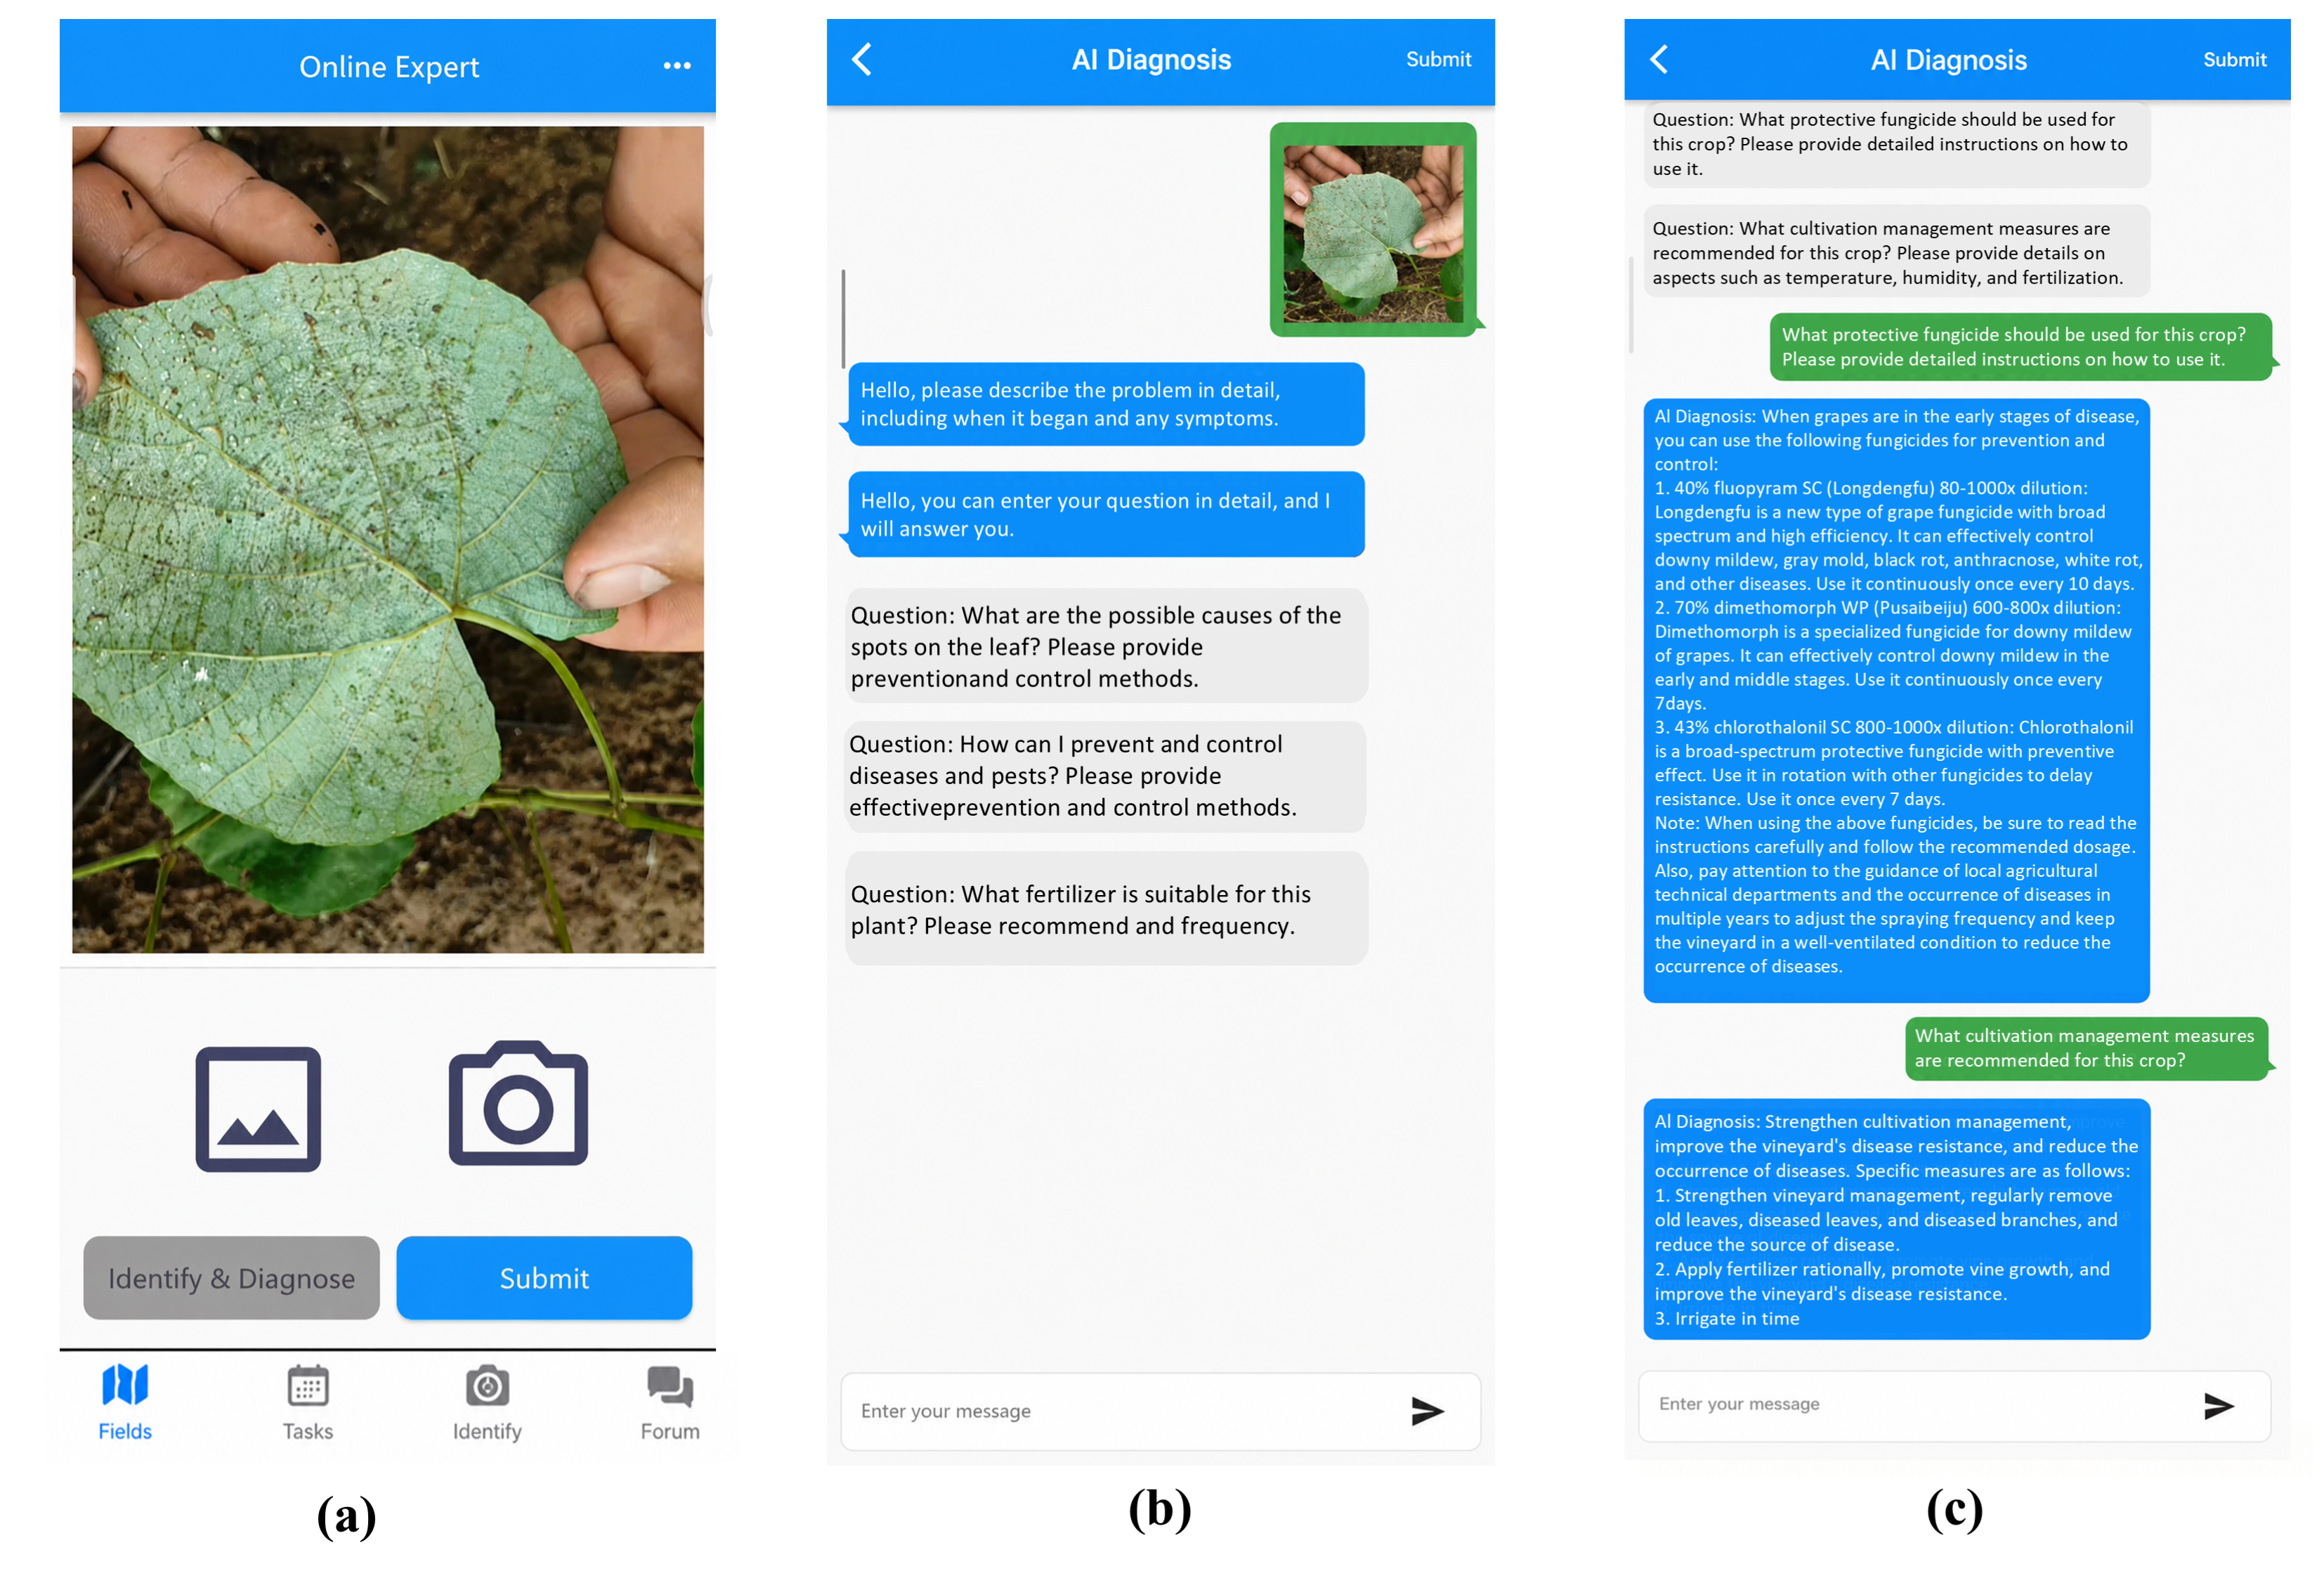
\includegraphics[width=\linewidth]{fig/ai_diagnosis_interfaces.png}
\caption[Symptom-image and advisory interfaces]{Symptom-image and advisory interfaces in GrapeMaster. (a) The image-upload page captures post-symptom visual information. (b) The result view provides classification output and follow-up questions. (c) The LLM-assisted interface streams management-oriented text. Record association depends on the field, crop, image, user, and message identifiers available to each function.}
\label{fig:ai_diagnosis_interfaces_result}
\end{figure}

\section{Implementation and deployment demonstration}\label{deployment-and-backend-record-audit}

\subsection{Software stack and deployment context}\label{software-stack-and-deployment-context}

The deployed GrapeMaster system combined a Flutter/Dart mobile client, a Django 4.2 and Django REST Framework backend, PostgreSQL persistence, scheduled jobs, Django Channels, and a separately deployed FastAPI disease service. Network dependencies supplied weather and geocoding, SMS or notification delivery, image classification, severity estimation, and streamed advisory interaction. The principal software stack is reported in Supplementary Table S5. This section uses retained deployment records and a representative record chain to demonstrate that the implemented architecture produced its intended business objects; it is not a controlled assessment of software usability or agronomic impact.

\subsection{Operational objects and representative workflow}\label{operational-objects-and-representative-workflow}

The backend export contained records created from 2023 to 2026, including field, crop, notification, and task resources. The mappable subset with field--crop linkage covered multiple vineyard regions, including subtropical grape-production areas in Guangxi and records from other production regions (Supplementary Figure S2).

The records were exported from the deployed platform rather than generated from simulated data. The tables were screened to identify accounts that contained both field and crop-management resources and to examine whether the business objects described in Sections~\ref{system-architecture}--\ref{features-and-functionalities} were present. Accounts without operational records, or without both field and crop records, were excluded according to the rules in Supplementary Tables S3 and S7.

The cleaned operational-record export contained 95 deduplicated registered accounts, of which 47 contained both field-creation records and crop-season management records and were retained as operational accounts. Within these accounts, the platform managed 139 vineyard fields and 128 crop seasons, generating 126 weather records, 126 phenology records, 252 disease-risk and model request--response records, 3,590 notification records, 151 plant-protection or irrigation tasks, and 234 fungicide or pesticide application records. Symptom and advisory records included 94 field notes or disease reports, 2,808 image-analysis records, 1,360 advisory or message records, and 27 forum records (Table~\ref{tab:backend_operational_coverage}). Of the retained field records, 124 had valid coordinates and crop-season linkage and were aggregated into 27 regions for spatial visualization.

A representative crop context containing weather, phenology, disease-risk, notification, completed plant-protection task, and fungicide product records was selected to illustrate the implemented workflow (Figure~\ref{fig:crop_season_replay_loop} and Supplementary Table S4). Weather, phenology, and disease request--response records shared the crop context. Notification and task records were also available within that context, while fungicide products were linked directly to operations through task identifiers. The replay therefore illustrates state updating, risk interpretation, event availability, task execution, and treatment feedback. It does not establish that the selected task was caused by a specific notification because the direct provenance key is absent. No field note or disease-incidence record was available for this case.

The retained objects support the software claim that GrapeMaster was implemented as more than a collection of analytical screens. They show backend persistence of crop state, model payloads, events, operations, and task-linked products. The record demonstration does not establish production efficacy, pesticide reduction, adoption, economic outcome, or the agronomic correctness of advisory text.

\begin{table}[H]
\centering
\begingroup
\setlength{\tabcolsep}{3pt}
\renewcommand{\arraystretch}{1.12}
\scriptsize
\caption{Operational-record coverage and crop-season-centered linkage in the retained GrapeMaster export.}
\label{tab:backend_operational_coverage}
\begin{minipage}{0.98\linewidth}
\begin{tabular}{p{0.21\linewidth} p{0.30\linewidth} p{0.22\linewidth} p{0.18\linewidth}}
\toprule
Demonstration level & Retained records & Linkage basis & Software interpretation \\
\midrule
Screened workflow set & 47 of 95 deduplicated accounts retained after screening & At least one field and one crop record & Accounts containing the principal setup objects \\
Field-season denominator & 139 fields and 128 crop seasons & Retained account, field UUID, and crop-season UUID & Field and crop-season records established as the audit base \\
Crop-season state records & 126 crop seasons with linked weather, phenology, disease-risk, and request-response payloads & Shared crop-season UUID & Environmental, phenological, and disease-risk states reconstructable by crop season \\
Event and operation records & 3590 notifications and 151 plant-protection or irrigation tasks & Retained user, field, or crop-season context & Event-delivery and field-operation records retained \\
Treatment-feedback records & 234 fungicide or pesticide records linked to 141 plant-protection tasks & Task UUID & Product records connected to completed or recorded task contexts \\
Symptom and advisory records & 94 field note or disease report records, 2808 image-analysis records, 1360 advisory or message records, and 27 forum records & Account, field, crop-season, image, or message identifiers & Symptom/advisory records retained, with completeness varying by season \\
Interpretation scope & No controlled production comparison in the backend export & Not applicable & No efficacy, pesticide-reduction, adoption, or economic outcome inferred \\
\bottomrule
\end{tabular}
\par\vspace{0.25em}{\raggedright\scriptsize Abbreviation: UUID, universally unique identifier.\par}
\end{minipage}
\endgroup
\end{table}

\begin{figure}[H]
\centering
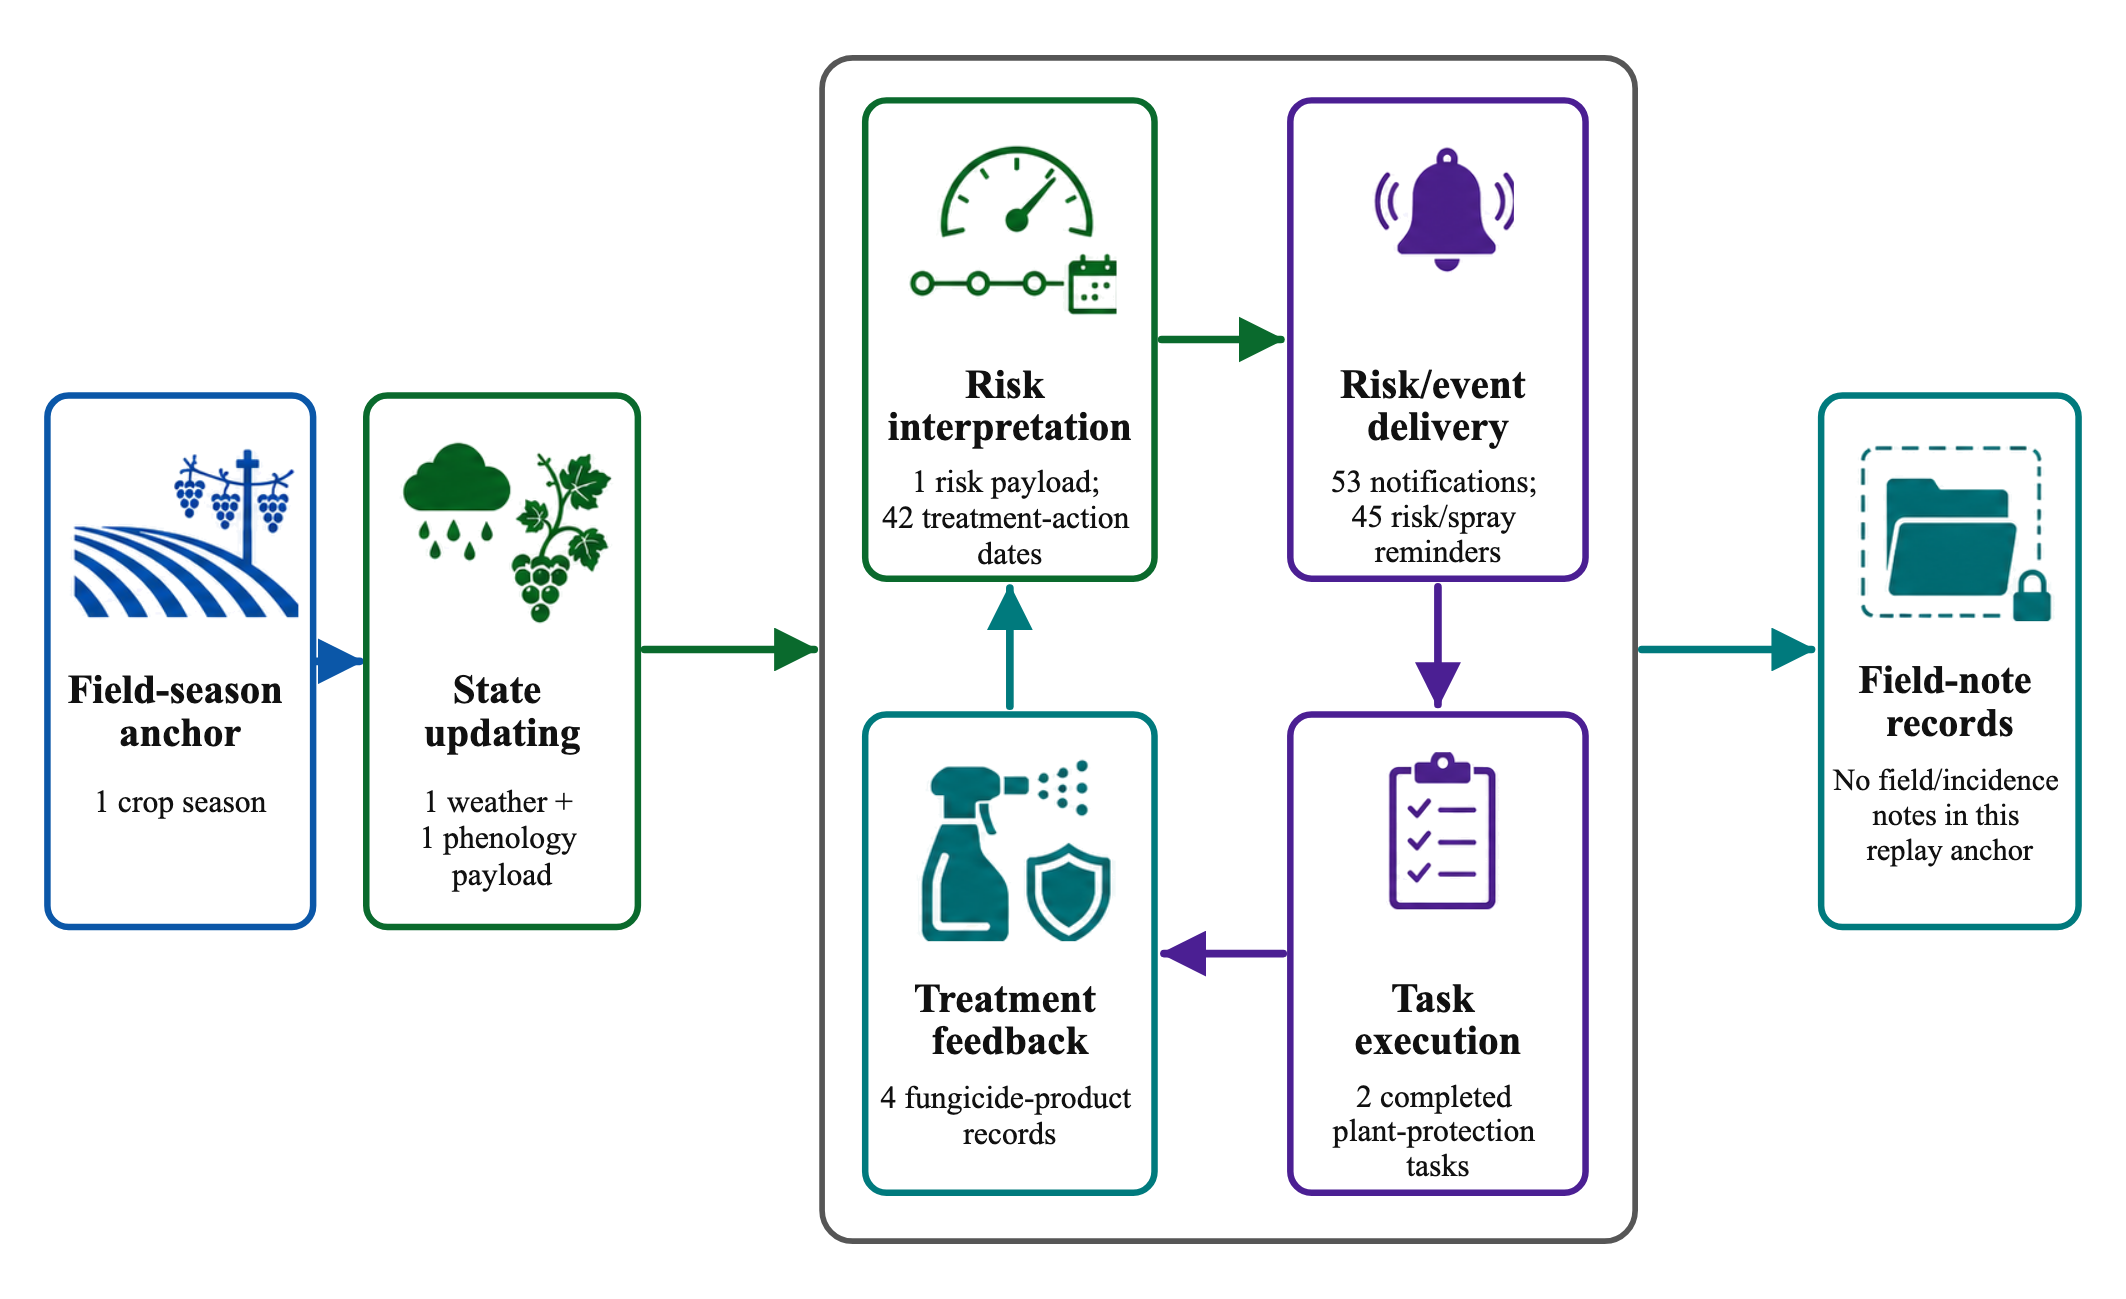
\includegraphics[width=\linewidth]{fig/disease_feedback_loop_frame_balanced_revised_figure_package/disease_feedback_loop_frame_balanced_revised_300dpi.png}
\caption[Record-level illustration of the risk-to-feedback workflow]{Record-level illustration of the risk-to-feedback workflow in GrapeMaster. Node labels indicate retained record counts for the selected crop context. Shared context supports reconstruction, while direct causal notification-to-task provenance is not asserted.}
\label{fig:crop_season_replay_loop}
\end{figure}

\subsection{Supporting analytical-component performance}\label{supporting-analytical-components}\label{evaluation-of-platform-compatible-analytical-modules}

Analytical components require evidence appropriate to their own outputs even though model development is not the primary contribution of this software paper. Independent results for the Guangxi phenology configuration, the FSIM-S first-infection configuration, and a grape disease image model are therefore retained as supporting component evidence (Table~\ref{tab:guangxi_field_data}). They do not evaluate the mobile application, backend architecture, deployment effectiveness, or production outcomes.

For the Guangxi broad-stage phenology module, the evaluation used 151 valid field observations from six Guangxi site-years. The module reached 58.0\% exact major-stage agreement and 76.0\% user-visible agreement after transition-window display, with a mean absolute stage distance of 0.45 major stages when the sparse post-harvest class was excluded from core metrics (Figure~\ref{fig:phenology_major_stage_validation_result}).

For the downy mildew risk-warning module, the FSIM-S configuration produced a validation mean absolute error of 6.3 days and a validation root mean square error of 6.5 days for first-infection timing (Figure~\ref{fig:core_analytical_support_result}). This result describes the evaluated Guangxi configuration of the platform-compatible risk module rather than the effectiveness of deployed plant-protection decisions.

For the grape disease image-recognition module, the evaluated model produced class-wise F1-scores from 0.926 to 0.998 across seven grape disease categories, with downy mildew reaching an F1-score of 0.986 (Figure~\ref{fig:core_analytical_support_result}). The LLM-assisted advisory component was not included in this module-evaluation section because no independent evaluation result for advisory quality was reported in this study.

\begin{table}[H]
\centering
\caption{Datasets used for platform-compatible analytical-module evaluation.}
\label{tab:guangxi_field_data}
\tablefontsize
\begin{tabular}{@{}p{0.24\linewidth} p{0.23\linewidth} p{0.16\linewidth} p{0.29\linewidth}@{}}
\toprule
Site or dataset & Cultivar or scope & Years & Data types \\
\midrule
Mingyang, Nanning & Jufeng & 2023, 2024 & Phenology observations, downy mildew monitoring, airborne sporangia monitoring, and management records \\
Du'an, Hechi & Maoputao Yeniang No. 2 & 2022, 2023, 2024 & Phenology observations, downy mildew monitoring, airborne sporangia monitoring, and management records \\
Xing'an, Guilin & Wenke & 2022 & Phenology observations, downy mildew monitoring, airborne sporangia monitoring, and management records \\
Grape disease image dataset & Multiple grape disease categories & Not based on site years & Symptom images \\
\bottomrule
\end{tabular}
\end{table}

\begin{figure}[H]
\centering
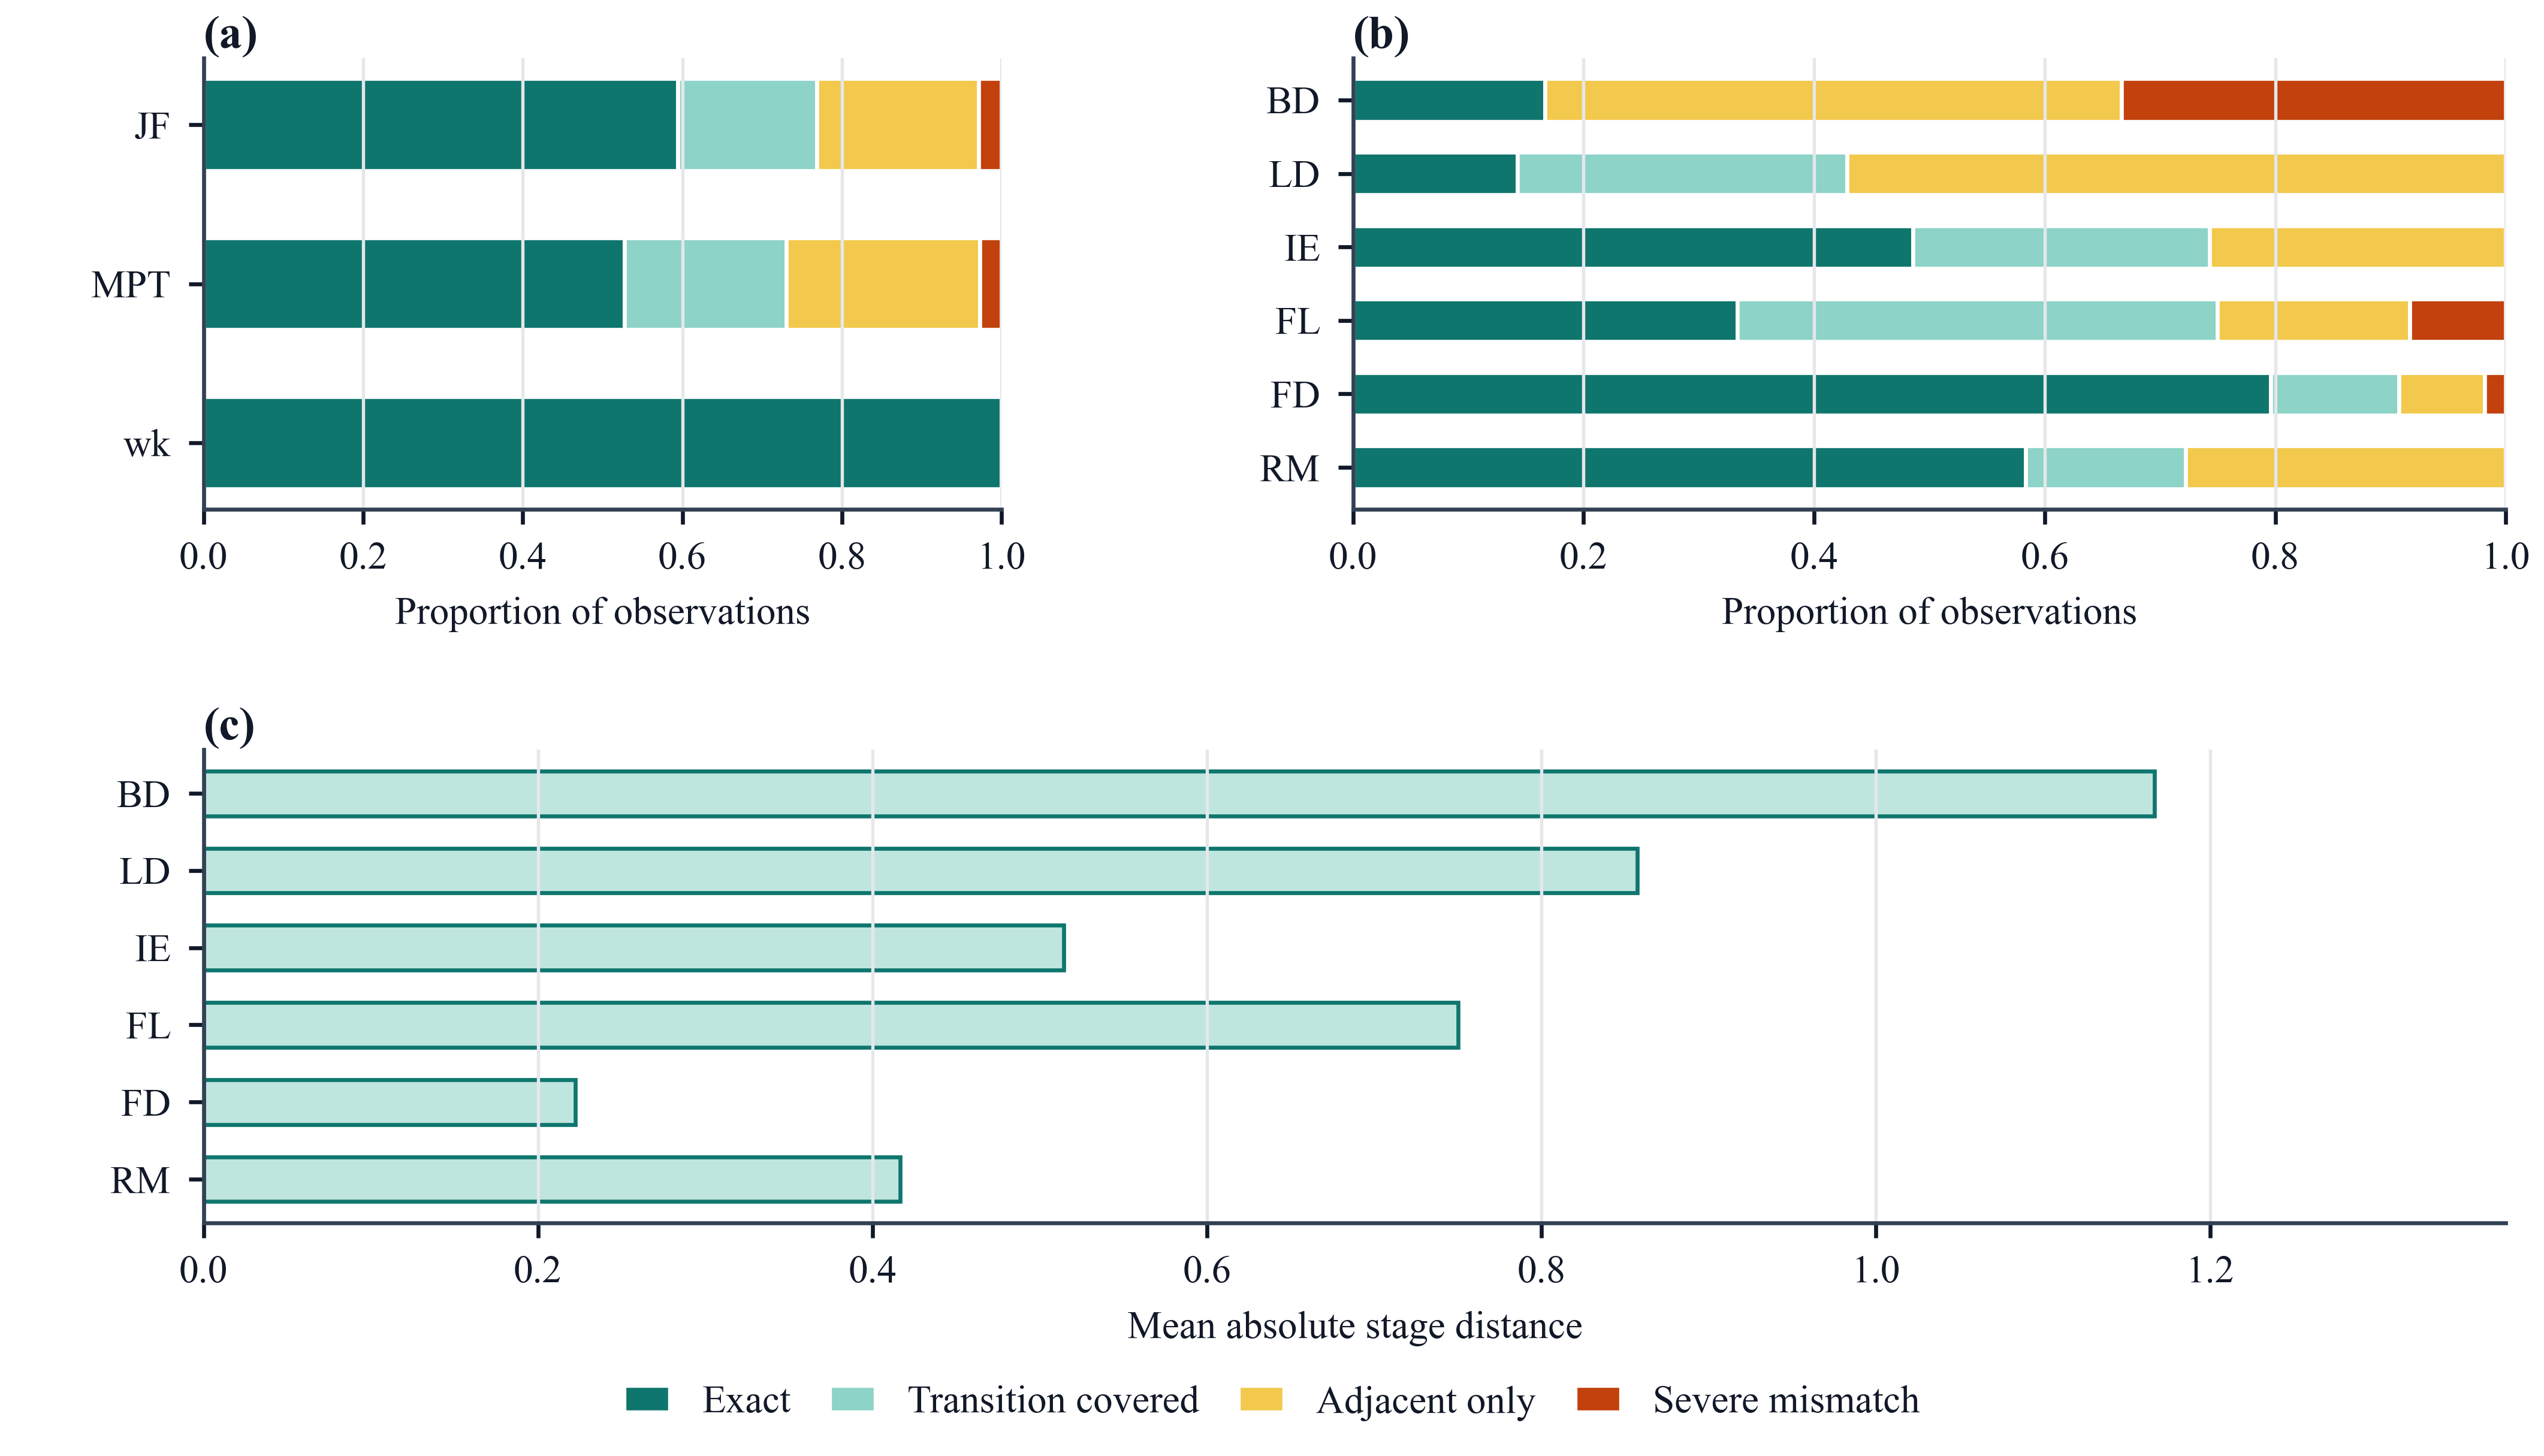
\includegraphics[width=\linewidth]{fig/phenology_major_stage_validation.png}
\caption[Validation results for the broad-stage phenology module]{Validation results for the platform-compatible broad-stage phenology module. (a) Outcome proportions are summarized by cultivar. (b) Outcome proportions are summarized by observed major stage. (c) Mean absolute stage distance is summarized by observed major stage. BD, bud development; LD, leaf development; IE, inflorescence emergence; FL, flowering; FD, fruit development; RM, ripening of berries.}
\label{fig:phenology_major_stage_validation_result}
\end{figure}

\begin{figure}[H]
\centering

\includegraphics[width=\linewidth]{fig/fsims_supporting_performance.png}
\caption[Module-level results for disease-risk and image-recognition components]{Module-level results for disease-risk and image-recognition components. (a) The FSIM-S panel reports validation error for downy mildew first-infection timing. (b) The image-recognition panel reports class-wise F1-scores for grape disease categories, with downy mildew highlighted.}
\label{fig:core_analytical_support_result}
\end{figure}

\section{Discussion}\label{discussion}

\subsection{Crop context as a software coordination mechanism}\label{crop-season-as-the-organizational-anchor-for-grapevine-disease-management}

The crop context is useful because vineyard software must represent two temporal scales. Fields provide stable geospatial and ownership identity, whereas weather, phenology, disease pressure, and management history change through time \citep{nogueirajuniorModellingDynamicsGrapevine2018,bregaglioPublicDecisionSupport2022}. GrapeMaster places changeable analytical and operational resources under a field-linked crop UUID rather than attaching every result only to a user or field. The deployment export demonstrates that this structure was used for weather, phenology, disease payloads, tasks, and products. The current object should nevertheless be understood as a software management context, not as a formally bounded agronomic season: explicit year, start, end, and lifecycle-state attributes are absent from the documented schema. Adding those attributes would strengthen archival separation and multi-year queries.

This design is less important as a claim that crop season is universally novel than as an implementation mechanism for coordinating heterogeneous services. It gives scheduled jobs, REST resources, and mobile controllers a common lookup key while preserving field identity above it. This follows broader digital-agriculture principles that call for coherent organization of data, models, and decisions \citep{romera2024digitalization,bakirScalableEndtoendIoT2026}.

\subsection{Integrating proactive and post-symptomatic services}\label{modular-platform-architecture-for-evolving-disease-management-systems}

GrapeMaster integrates analytical services according to their operational role rather than treating all models as equivalent predictors. Weather and phenology establish environmental and host state. The disease service supports pre-symptomatic risk interpretation and treatment timing. Image recognition supplies post-symptomatic visual evidence. LLM-assisted interaction supplies explanation and follow-up consultation. This role-based separation is valuable because it allows the primary disease workflow to remain available independently of the image and language services and allows analytical components to be calibrated or redeployed without embedding their algorithms in the mobile client.

The service boundaries are not equally mature. The disease service has a typed request schema and stateless API, while the backend owns persistence and management linkage. The hosted image and advisory interfaces are parsed directly by large frontend screens and are configured through fixed network locations in the current client. Their expected message contracts are therefore more tightly coupled to the current frontend. Replacing them would require either preserving response wording and stream markers or introducing stable versioned adapters. The architecture supports model separation conceptually, but future implementations should add service discovery, configuration management, contract tests, and version metadata before claiming broad plug-and-play extensibility.

\subsection{From model output to field-management functions}\label{from-analytical-outputs-to-executable-disease-management-records}

The software contribution is clearest in the treatment-feedback path. An analytical result gains operational value when the application exposes it through warnings and tasks and when completed operations can alter the state used for later interpretation \citep{rossiAddressingImplementationProblem2014,rossiSharingDecisionmakingTools2023}. GrapeMaster retains disease request--response payloads, presents risk and warning information, stores task execution and product records, translates fungicide history into the disease-service schema, and reruns supported calculations. This design extends model delivery toward management-aware software operation.

The distinction between contextual and causal linkage remains important. Product records have direct task relationships, and weather, phenology, and disease payloads have crop relationships. Notifications and tasks can be retrieved within the same context, but the task schema does not record its originating notification. The software can therefore reconstruct co-occurring stages of the risk-to-action pathway but cannot prove from the database alone that one warning caused one operation. A future provenance key linking source event, created task, user modification, execution, and model version would make the workflow fully auditable.

\subsection{Limitations and future software development}\label{limitations-and-future-directions}

This paper documents a developed software system, its functions, and its analytical integrations. It does not establish disease-control efficacy, fungicide-use efficiency, economic benefit, usability, or adoption \citep{rossiAddressingImplementationProblem2014,roseDecisionSupportTools2016}. The operational export demonstrates implemented record coverage but is not a controlled field trial. Regional deployment also requires calibration and validation of analytical components for local weather, cultivars, epidemiology, and management \citep{bregaglioPublicDecisionSupport2022}.

Several implementation limitations affect reproducibility and future maintenance. The crop object lacks explicit lifecycle fields. The backend uses hard-coded external dependencies in several paths, starts scheduled work during module import, and has limited automated tests. Some WebSocket state is held in memory, which constrains multi-instance deployment. The active disease-service source and the separately reported FSIM-S validation do not yet share an archived immutable deployment identifier. The image and advisory services are external to the principal backend repository, and the available source does not provide the hosted LLM checkpoint, fine-tuning data, prompt, or version. LLM advisory quality was not independently evaluated. These limitations do not remove the implemented software functions, but they bound claims of reproducibility, reliability, scalability, and advisory validity.

Priority future work is therefore software-focused: archive versioned frontend, backend, disease, image, and LLM artifacts; replace fixed endpoints with configurable adapters; add API-contract and end-to-end tests; add explicit crop-season lifecycle fields and event-to-task provenance; evaluate LLM advice for factuality and safety; and then conduct repeated user and field studies to assess usability and agronomic outcomes.

\section{Conclusion}\label{conclusion}

This paper presented GrapeMaster as an agricultural software system for integrating vineyard disease models with field-management functions. A Flutter mobile client and Django backend organize field and crop context, scheduled weather and phenology processing, stateless disease-service calls, warnings, tasks, products, image diagnosis, and LLM-assisted advisory interaction. The crop-context architecture separates persistent field identity from changeable analytical and operational state, while retained request--response and task--product relationships support later review.

The principal integration contribution is the risk-to-action-to-feedback workflow: disease inputs and outputs are retained by the backend, model results enter user-facing event and task functions, and recorded fungicide applications are translated into management-history input for supported recalculation. The image-recognition and LLM branch provides a complementary post-symptomatic workflow. Deployment records and component results demonstrate implemented use and analytical compatibility, while the stated limitations define where stronger provenance, versioning, testing, and LLM validation are still required. GrapeMaster therefore provides a concrete software design for combining heterogeneous agricultural models and management services within one vineyard application.

\section*{CRediT authorship contribution statement}

To be completed before submission.

\section*{Declaration of competing interest}

The authors declare that they have no known competing financial interests or personal relationships that could have appeared to influence the work reported in this paper.

\section*{Data availability}

The de-identified derived datasets and analysis scripts supporting the figures, tables, and summary statistics reported in this study are available from the corresponding author upon reasonable request. These materials include operational-record summaries, representative workflow replay summaries, phenology validation results, disease-risk timeline data, figure source data, and the scripts used for data summarization and visualization.

Raw operational records from the deployed GrapeMaster platform are not publicly available because they contain user account information, field locations, uploaded images, messages, task records, and other management data subject to privacy and confidentiality restrictions. De-identified data supporting the reported analyses are available from the corresponding author upon reasonable request, subject to applicable privacy and confidentiality requirements.

\section*{Software availability}

The GrapeMaster mobile client, application backend, and disease-service source are maintained in the research group's software repositories. Source snapshots corresponding to the implementation documented in this paper are available from the corresponding author upon reasonable request. A submission archive should include versioned releases of the frontend, backend, disease service, configuration files, API contracts, and deployment instructions. The separately hosted image-recognition and LLM advisory artifacts require their own version and availability statements because they are not fully contained in the principal backend repository.

\section*{Acknowledgements}

To be completed before submission.

\section*{Ethics and user data privacy statement}

The operational records used in this study were analyzed in aggregated or de-identified form, and no personally identifiable user information is reported.

\section*{Supplementary material}

Supplementary material associated with this article is provided as a separate file.

\bibliographystyle{elsarticle-harv}
\bibliography{reference/Grape}

\end{document}
